\chapter{HASIL DAN PEMBAHASAN}

\section{Hasil Penelitian}
Penelitian ini membandingkan kinerja Hadoop dan Spark pada \textit{platform cloud} DigitalOcean menggunakan alat pengujian data besar yang bernama HiBench pada lingkup \textit{Micro Benchmarks}, yaitu \textit{Word Count} dan \textit{Sort} dengan data masukan berupa teks.
Setiap pengujian, nilai execution time (waktu eksekusi) memiliki satuan detik dan nilai \textit{throughput} memiliki satuan megabita per detik. Ukuran data input akan diubah secara bertahap untuk merepresentasikan berbagai ukuran data pada dunia nyata.

\subsection {Persebaran Waktu Eksekusi pada Hadoop dan Spark}
Waktu eksekusi adalah waktu yang diperlukan dalam memproses data. Nilai parameter ini didapatkan dengan cara mencari selisih antara waktu awal dan waktu akhir saat Apache Hadoop dan Apache Spark dijalankan atau dihentikan untuk memproses input data dengan beban kerja masing-masing. Satuan pengukuran untuk parameter waktu eksekusi adalah detik atau \textit{seconds}. Setiap beban kerja dijalankan sebanyak 5x untuk mendapatkan hasil yang lebih terukur. 

\begin{figure}[h]
    \centering
    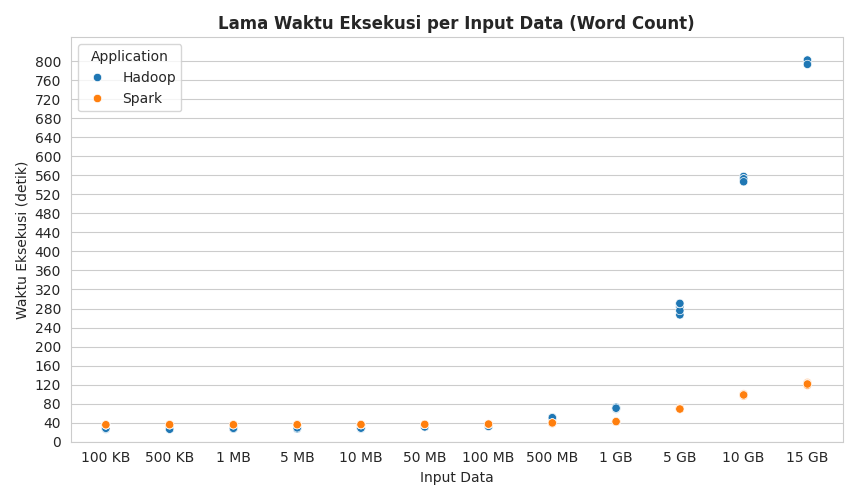
\includegraphics[width=1\textwidth]{figures/ch04/1-lama-waktu-eksekusi-wordcount.png}
    \caption{Persebaran Waktu Eksekusi \textit{Word Count} (Hadoop, Spark)}
    \label{fig:lama-waktu-eksekusi-wordcount}
\end{figure}

Gambar \ref{fig:lama-waktu-eksekusi-sort} dan \ref{fig:lama-waktu-eksekusi-wordcount} menyajikan scatter plot yang membandingkan performa Hadoop dan Spark dalam dua tugas pemrosesan data yang berbeda: sorting dan word count.  Sumbu x pada kedua gambar menunjukkan variasi ukuran input data, mulai dari 100 KB hingga 15 GB, sedangkan sumbu y menunjukkan waktu eksekusi dalam detik.

Pada Gambar \ref{fig:lama-waktu-eksekusi-sort}, terlihat bahwa Spark secara konsisten mengungguli Hadoop dalam tugas sorting. Titik data Spark selalu berada di bawah titik data Hadoop, menunjukkan waktu eksekusi yang lebih singkat untuk semua ukuran data. Perbedaan performa ini semakin signifikan seiring bertambahnya ukuran data. Sebagai contoh, pada ukuran data 15 GB, Spark menyelesaikan tugas sorting dalam waktu kurang dari 240 detik, sedangkan Hadoop membutuhkan waktu lebih dari 360 detik. Selain itu, titik data Spark lebih rapat, mengindikasikan variabilitas performa yang lebih rendah dan menghasilkan waktu eksekusi yang lebih konsisten.

Pada Gambar \ref{fig:lama-waktu-eksekusi-wordcount}, Spark masih menunjukkan performa yang lebih baik daripada Hadoop pada sebagian besar ukuran data. Namun, perbedaan performanya tidak sebesar pada tugas sorting. Pada ukuran data kecil (di bawah 1 GB), kedua framework menunjukkan waktu eksekusi yang relatif sama. Pada ukuran data yang lebih besar, Spark tetap lebih cepat, kecuali pada 15 GB di mana Hadoop menunjukkan waktu eksekusi yang sedikit lebih cepat, namun dengan variabilitas yang lebih tinggi. 

Secara keseluruhan, hasil ini menunjukkan bahwa Spark umumnya lebih unggul dan konsisten daripada Hadoop dalam menangani tugas pemrosesan data, terutama untuk sorting. Namun, perbandingan performa dapat bervariasi tergantung pada jenis tugas dan ukuran data.

\begin{figure}[h]
    \centering
    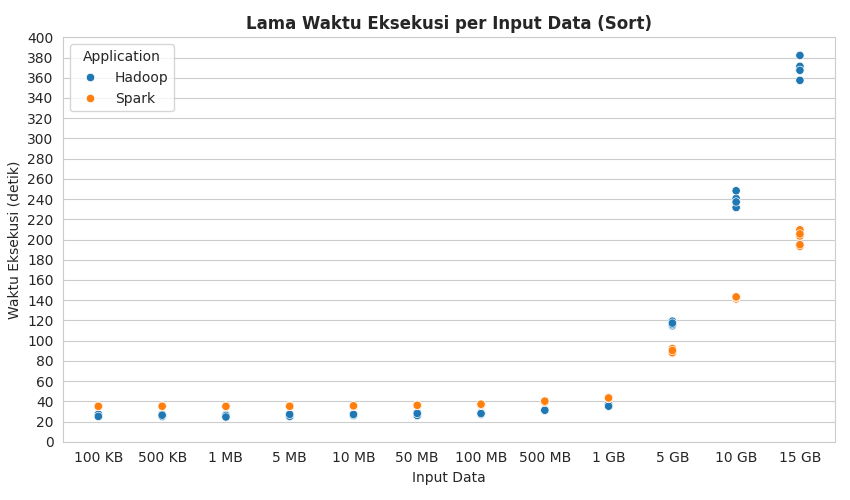
\includegraphics[width=1\textwidth]{figures/ch04/1-lama-waktu-eksekusi-sort.png}
    \caption{Persebaran Waktu Eksekusi \textit{Sort} (Hadoop, Spark)}
    \label{fig:lama-waktu-eksekusi-sort}
\end{figure}


\subsection {Persebaran \textit{Throughput} pada Hadoop dan Spark}

\begin{figure}[h]
    \centering
    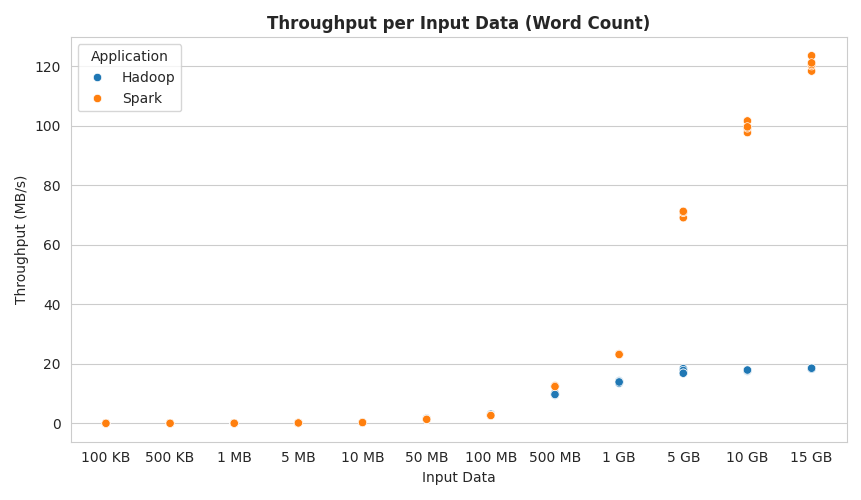
\includegraphics[width=1\textwidth]{figures/ch04/1-throughput-wordcount.png}
    \caption{\textit{Throughput Word Count} (Hadoop, Spark)}
    \label{fig:throughput-wordcount}
\end{figure}
Kedua gambar di atas menyajikan scatter plot yang membandingkan throughput Hadoop dan Spark dalam dua tugas pemrosesan data: sorting (Gambar \ref{fig:throughput-sort}) dan word count (Gambar \ref{fig:throughput-wordcount}). Sumbu x pada kedua gambar menunjukkan variasi ukuran input data, sedangkan sumbu y menunjukkan throughput dalam MB/s. 

Pada tugas sorting (Gambar \ref{fig:throughput-sort}), Spark menunjukkan peningkatan throughput yang signifikan seiring dengan bertambahnya ukuran data. Pada ukuran data terbesar (15 GB), Spark mencapai throughput sekitar 40 MB/s. Sebaliknya, Hadoop menunjukkan peningkatan throughput yang lebih lambat dan hanya mencapai sekitar 35 MB/s pada ukuran data yang sama. Hal ini menunjukkan bahwa Spark mampu memanfaatkan sumber daya secara lebih efisien untuk memproses data dalam jumlah besar.

Pada tugas word count (Gambar \ref{fig:throughput-wordcount}), Spark mencapai throughput yang lebih tinggi daripada Hadoop untuk sebagian besar ukuran data. Perbedaan throughput paling mencolok terlihat pada ukuran data menengah (100 MB - 1 GB), di mana Spark mencapai throughput lebih dari 15 MB/s, sedangkan Hadoop hanya mencapai sekitar 5 MB/s. Meskipun Hadoop menunjukkan peningkatan throughput yang signifikan pada ukuran data terbesar (15 GB), mendekati throughput Spark, Spark tetap memiliki keunggulan dalam efisiensi pemrosesan data, terutama untuk ukuran data yang lebih kecil.

Hasil ini menunjukkan bahwa Spark secara umum lebih efisien dalam memanfaatkan sumber daya untuk memproses data dalam jumlah besar dibandingkan dengan Hadoop, baik untuk tugas sorting maupun word count.
\begin{figure}[h]
    \centering
    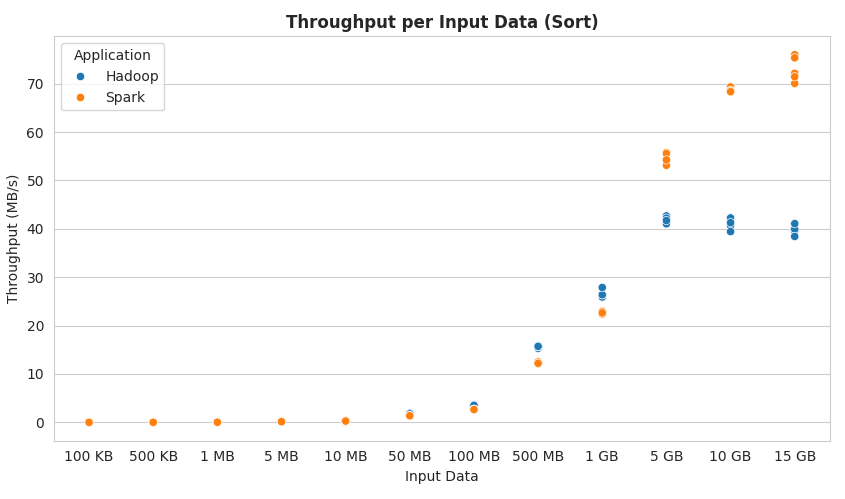
\includegraphics[width=1\textwidth]{figures/ch04/1-throughput-sort.png}
    \caption{\textit{Throughput Sort} (Hadoop, Spark)}
    \label{fig:throughput-sort}
\end{figure}

\subsection {Rata-rata Waktu Eksekusi pada Hadoop dan Spark}
Gambar \ref{fig:mean-dur-sort} dan \ref{fig:mean-dur-wordcount} menyajikan line plot yang menggambarkan rata-rata waktu eksekusi Hadoop dan Spark untuk tugas sorting dan word count dengan berbagai ukuran data. Sumbu x pada kedua gambar menunjukkan ukuran input data, sedangkan sumbu y menunjukkan rata-rata waktu eksekusi dalam detik. Garis vertikal pada kedua gambar menunjukkan titik di mana Spark mulai menunjukkan performa yang lebih cepat dibandingkan Hadoop.

Pada Gambar \ref{fig:mean-dur-sort}, terlihat bahwa Spark secara konsisten lebih cepat daripada Hadoop untuk semua ukuran data pada tugas sorting. Perbedaan performa semakin signifikan seiring dengan bertambahnya ukuran data. Titik di mana Spark mulai mengungguli Hadoop terjadi pada ukuran data 1 GB. Pada titik ini, waktu eksekusi Spark mulai menurun secara signifikan dibandingkan dengan Hadoop yang meningkat secara eksponensial.

Pada Gambar \ref{fig:mean-dur-wordcount}, Spark juga menunjukkan performa yang lebih baik daripada Hadoop pada sebagian besar ukuran data pada tugas word count. Perbedaan performa mulai terlihat pada ukuran data 100 MB, dan Spark terus unggul hingga ukuran data terbesar (15 GB). 

\begin{figure}[h]
    \centering
    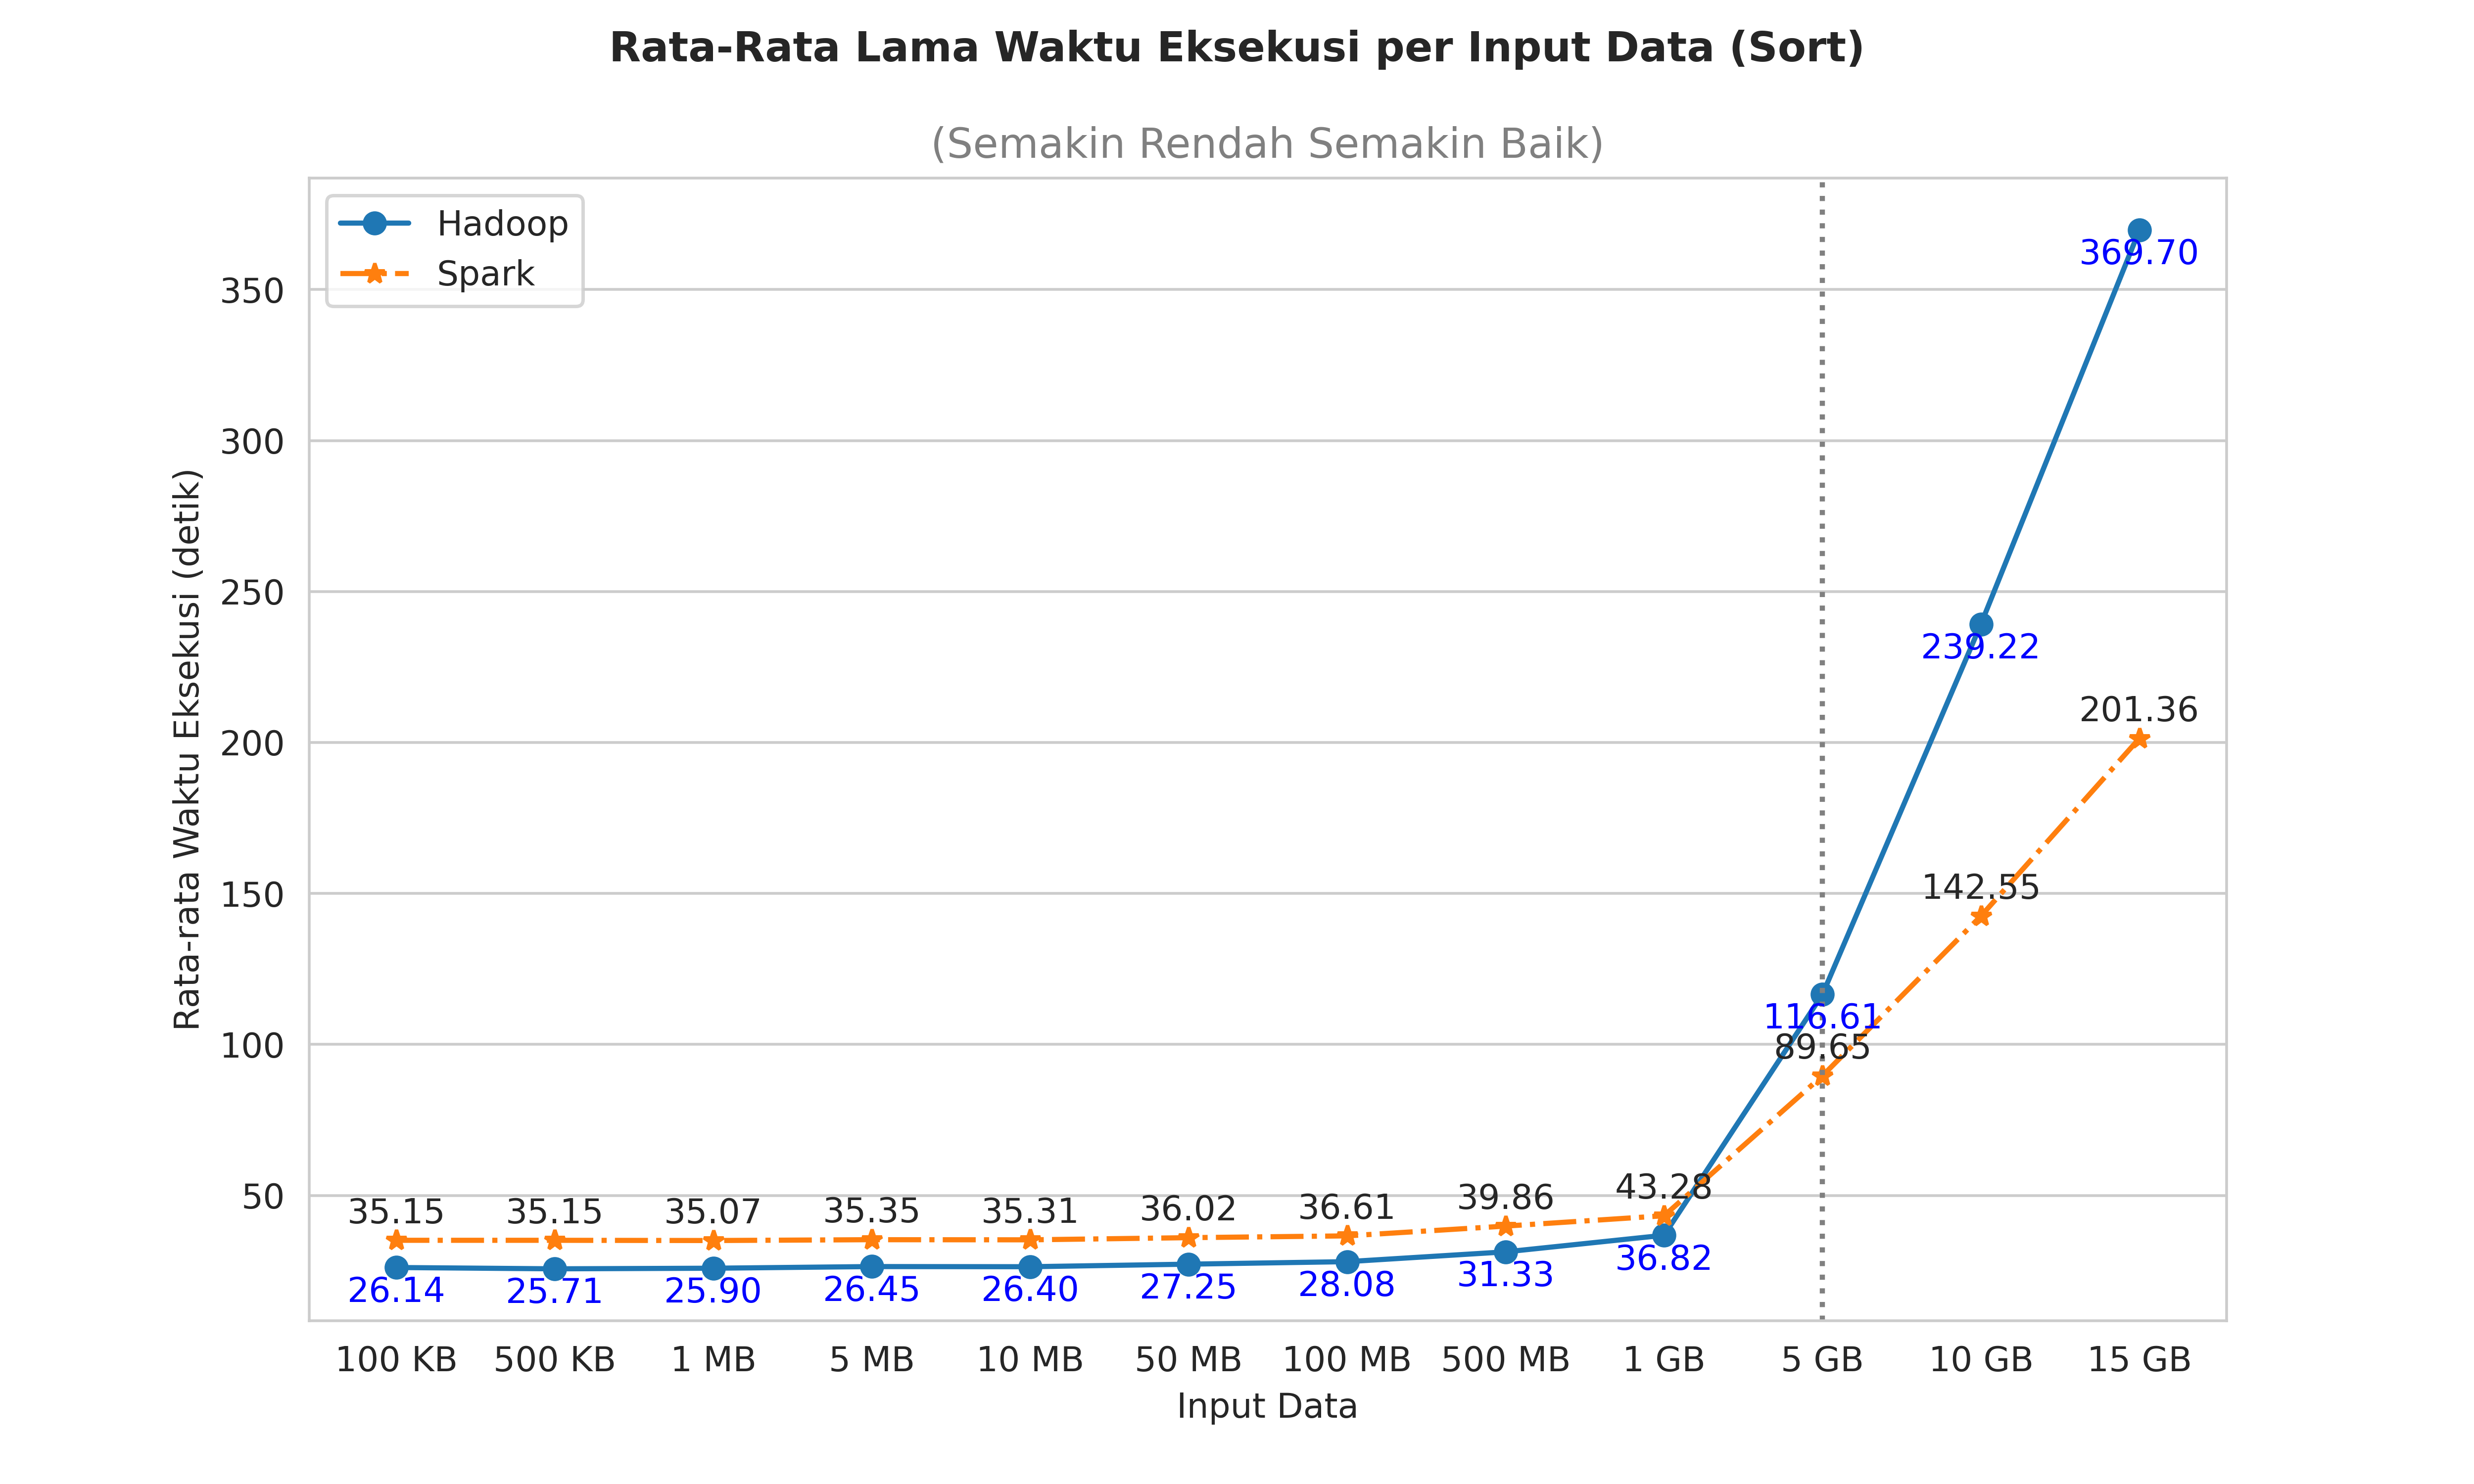
\includegraphics[width=1\textwidth]{figures/ch04/2-mean-lama-waktu-eksekusi-sort.png}
    \caption{Rata-rata Waktu Eksekusi \textit{(Sort)}}
    \label{fig:mean-dur-sort}
\end{figure}

\begin{figure}[h]
    \centering
    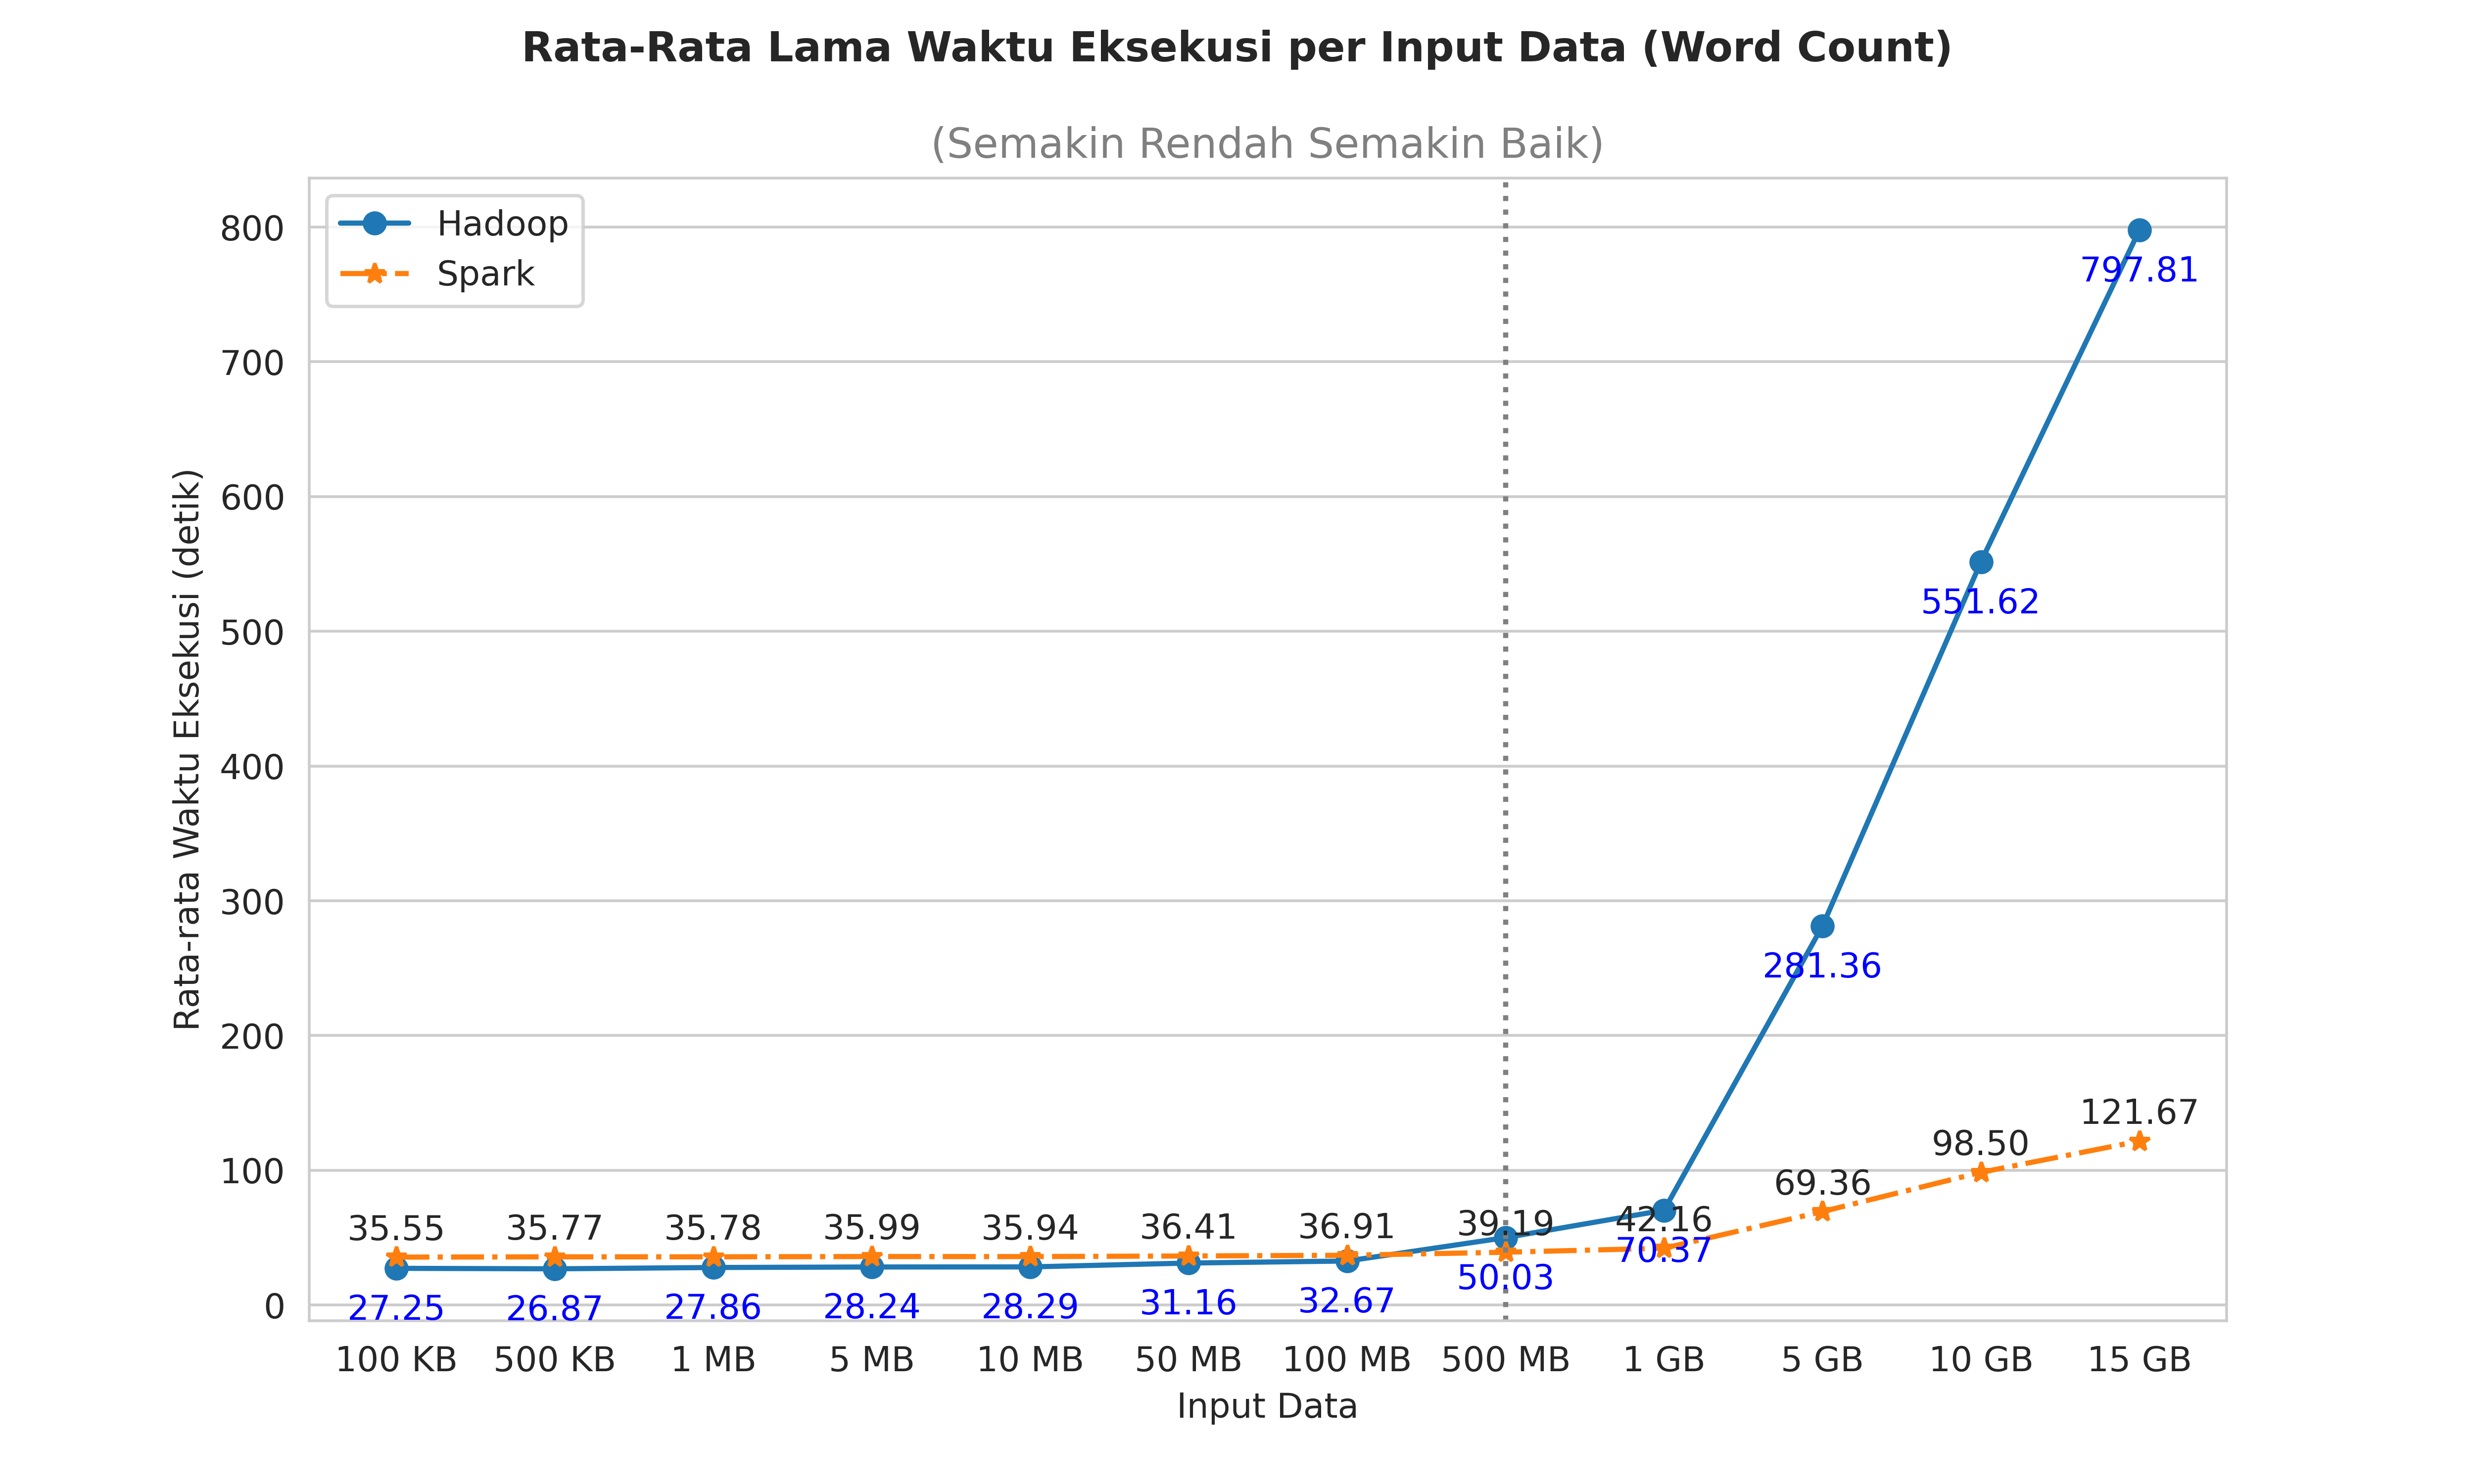
\includegraphics[width=1\textwidth]{figures/ch04/2-mean-lama-waktu-eksekusi-wordcount.png}
    \caption{Rata-rata Waktu Eksekusi \textit{(Word Count)}}
    \label{fig:mean-dur-wordcount}
\end{figure}

\subsection {Rata-rata Throughput pada Hadoop dan Spark}

Gambar \ref{fig:mean-throughput-sort} dan \ref{fig:mean-throughput-wordcount} menyajikan line plot yang menggambarkan rata-rata throughput Hadoop dan Spark untuk tugas sorting dan word count dengan berbagai ukuran data. Sumbu x pada kedua gambar menunjukkan ukuran input data, sedangkan sumbu y menunjukkan rata-rata throughput dalam MB/s. Garis vertikal pada kedua gambar menunjukkan titik di mana Spark mulai menunjukkan throughput yang lebih tinggi dibandingkan Hadoop.

Pada tugas sorting, Spark menunjukkan peningkatan throughput yang signifikan seiring dengan meningkatnya ukuran data. Pada ukuran data kecil (di bawah 500 MB), throughput Hadoop dan Spark relatif rendah dan sebanding. Namun, setelah titik 500 MB, Spark secara konsisten menunjukkan throughput yang lebih tinggi, mencapai 68.68 MB/s pada 15 GB dibandingkan dengan 45.39 MB/s untuk Hadoop. 

Pada tugas word count, Spark juga mengungguli Hadoop dalam hal throughput, meskipun dengan perbedaan yang tidak sebesar pada tugas sorting. Spark mulai menunjukkan throughput yang lebih tinggi pada ukuran data 100 MB.  Pada ukuran data 15 GB, Spark mencapai throughput 99.405 MB/s, sedangkan Hadoop hanya mencapai 18.407 MB/s.

\begin{figure}[h]
    \centering
    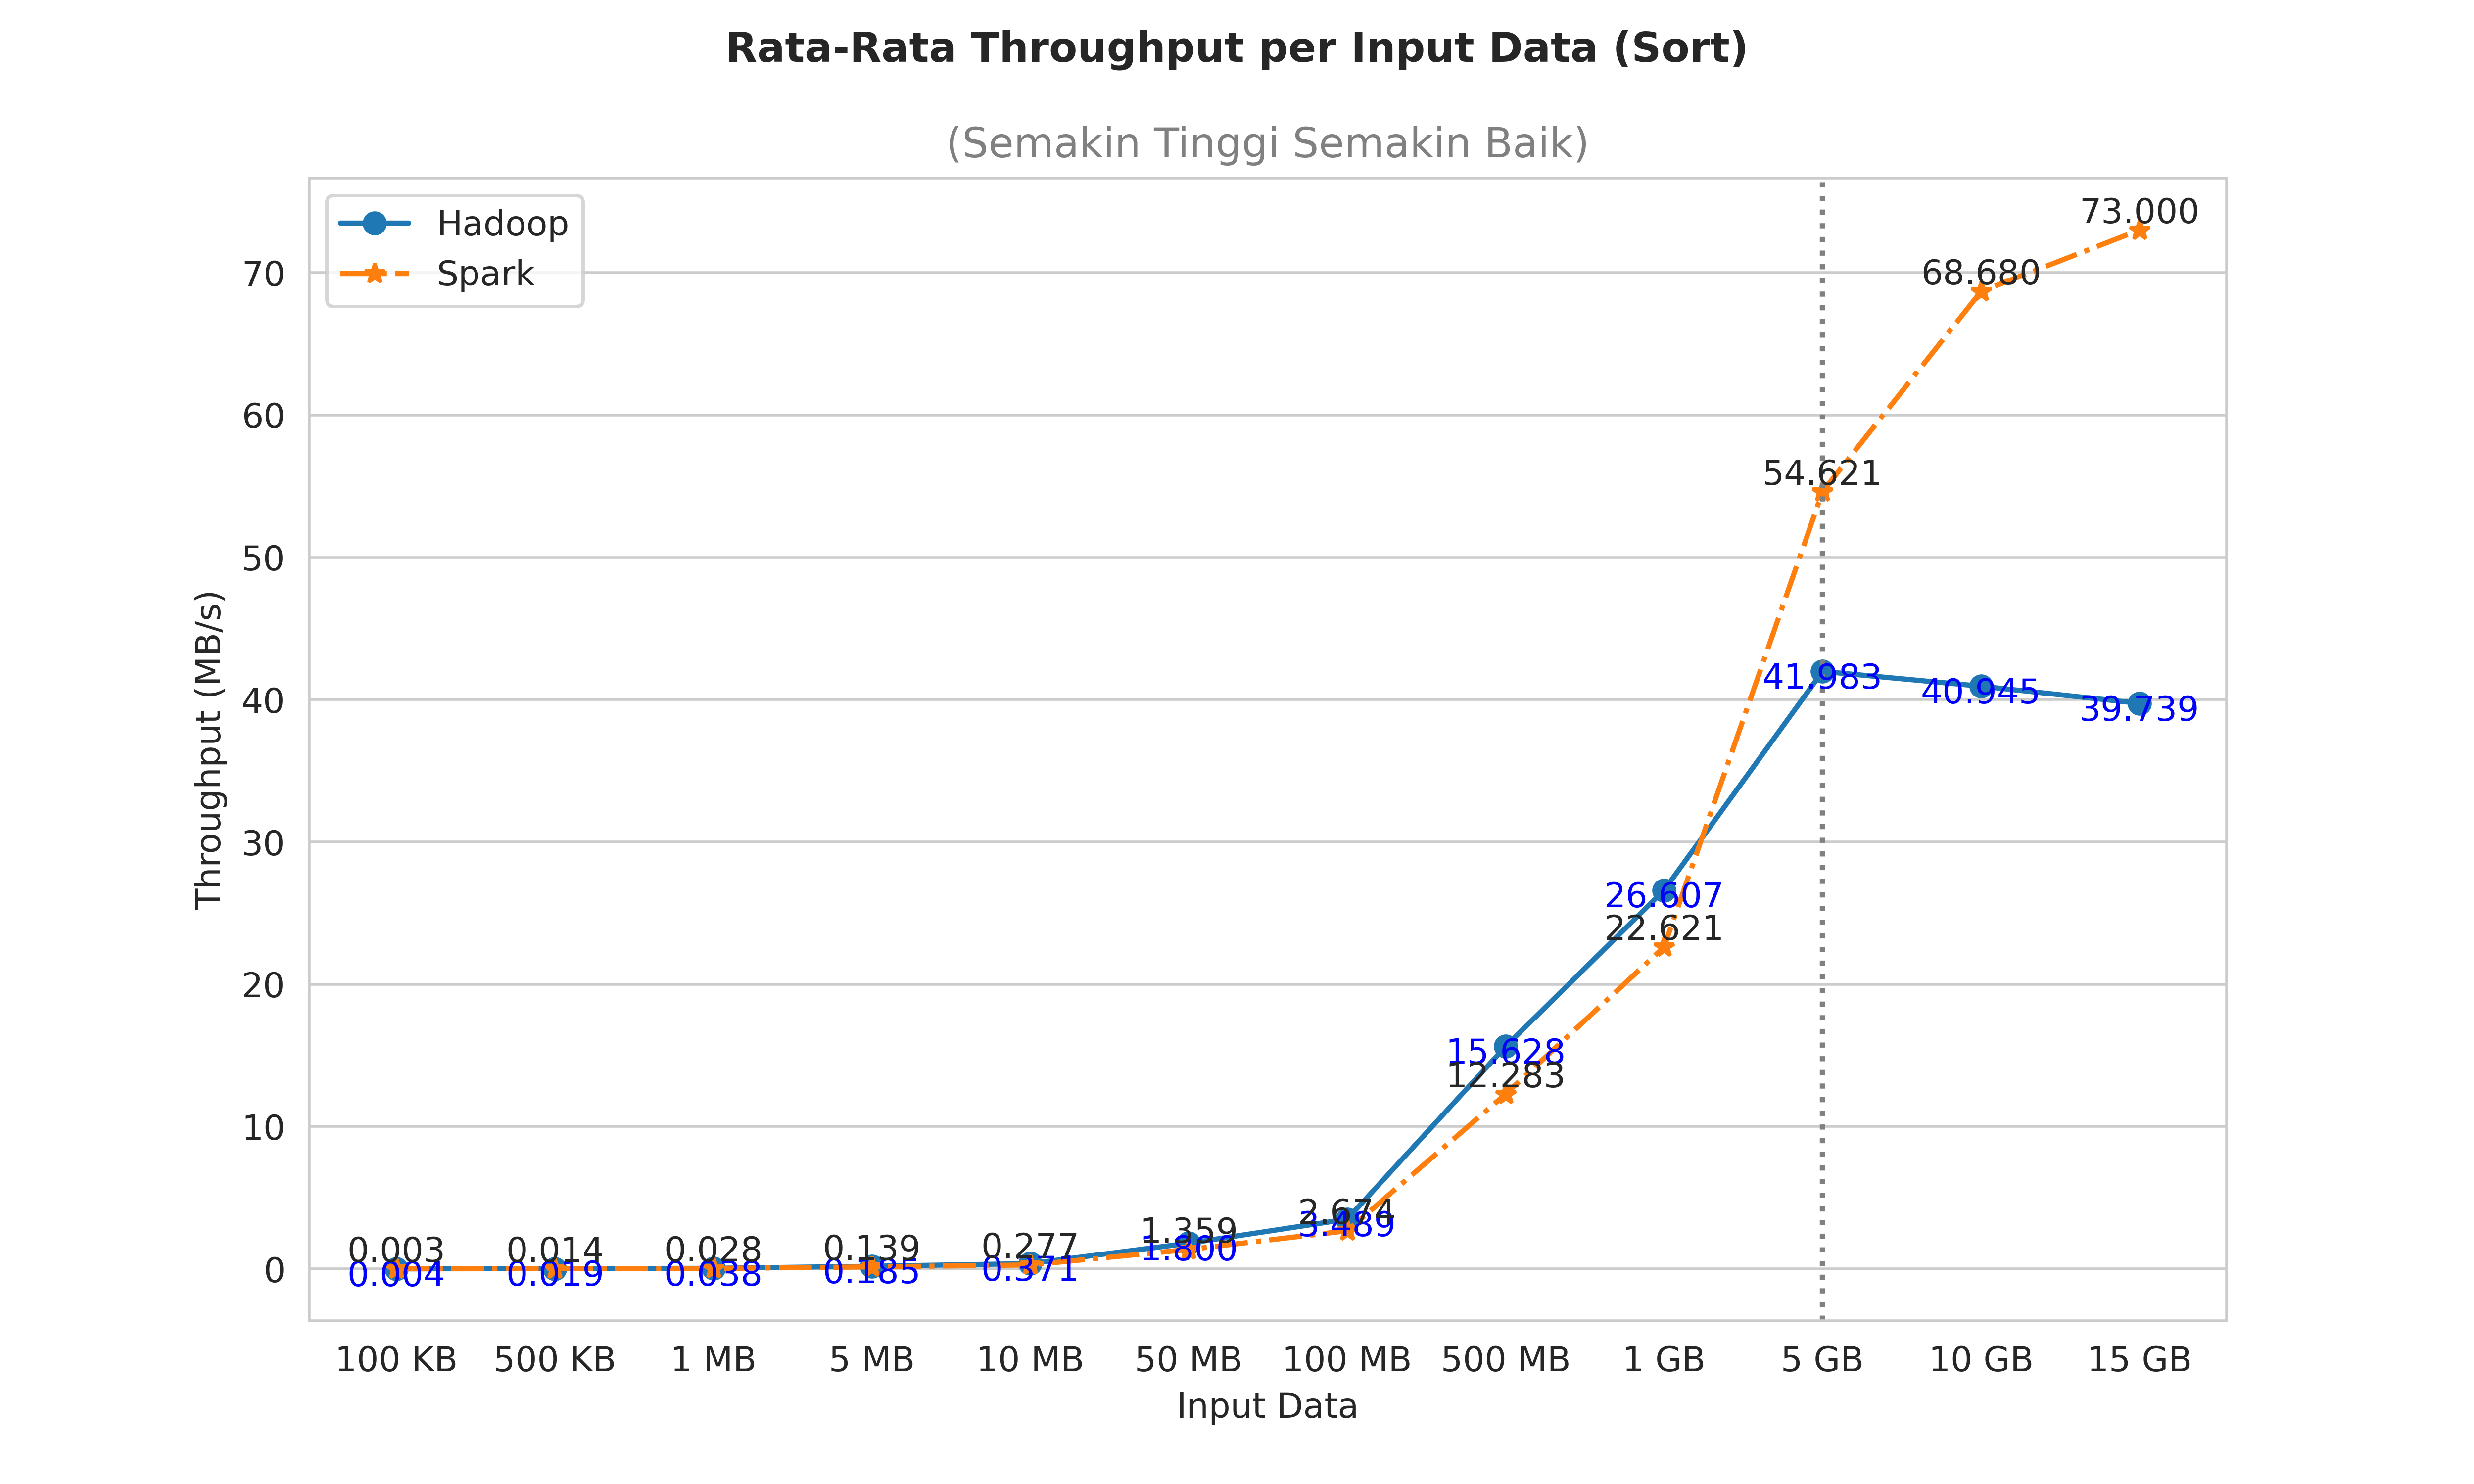
\includegraphics[width=1\textwidth]{figures/ch04/2-mean-throughput-sort.png}
    \caption{Rata-rata \textit{Throughput (Sort)}}
    \label{fig:mean-throughput-sort}
\end{figure}

\begin{figure}[h]
    \centering
    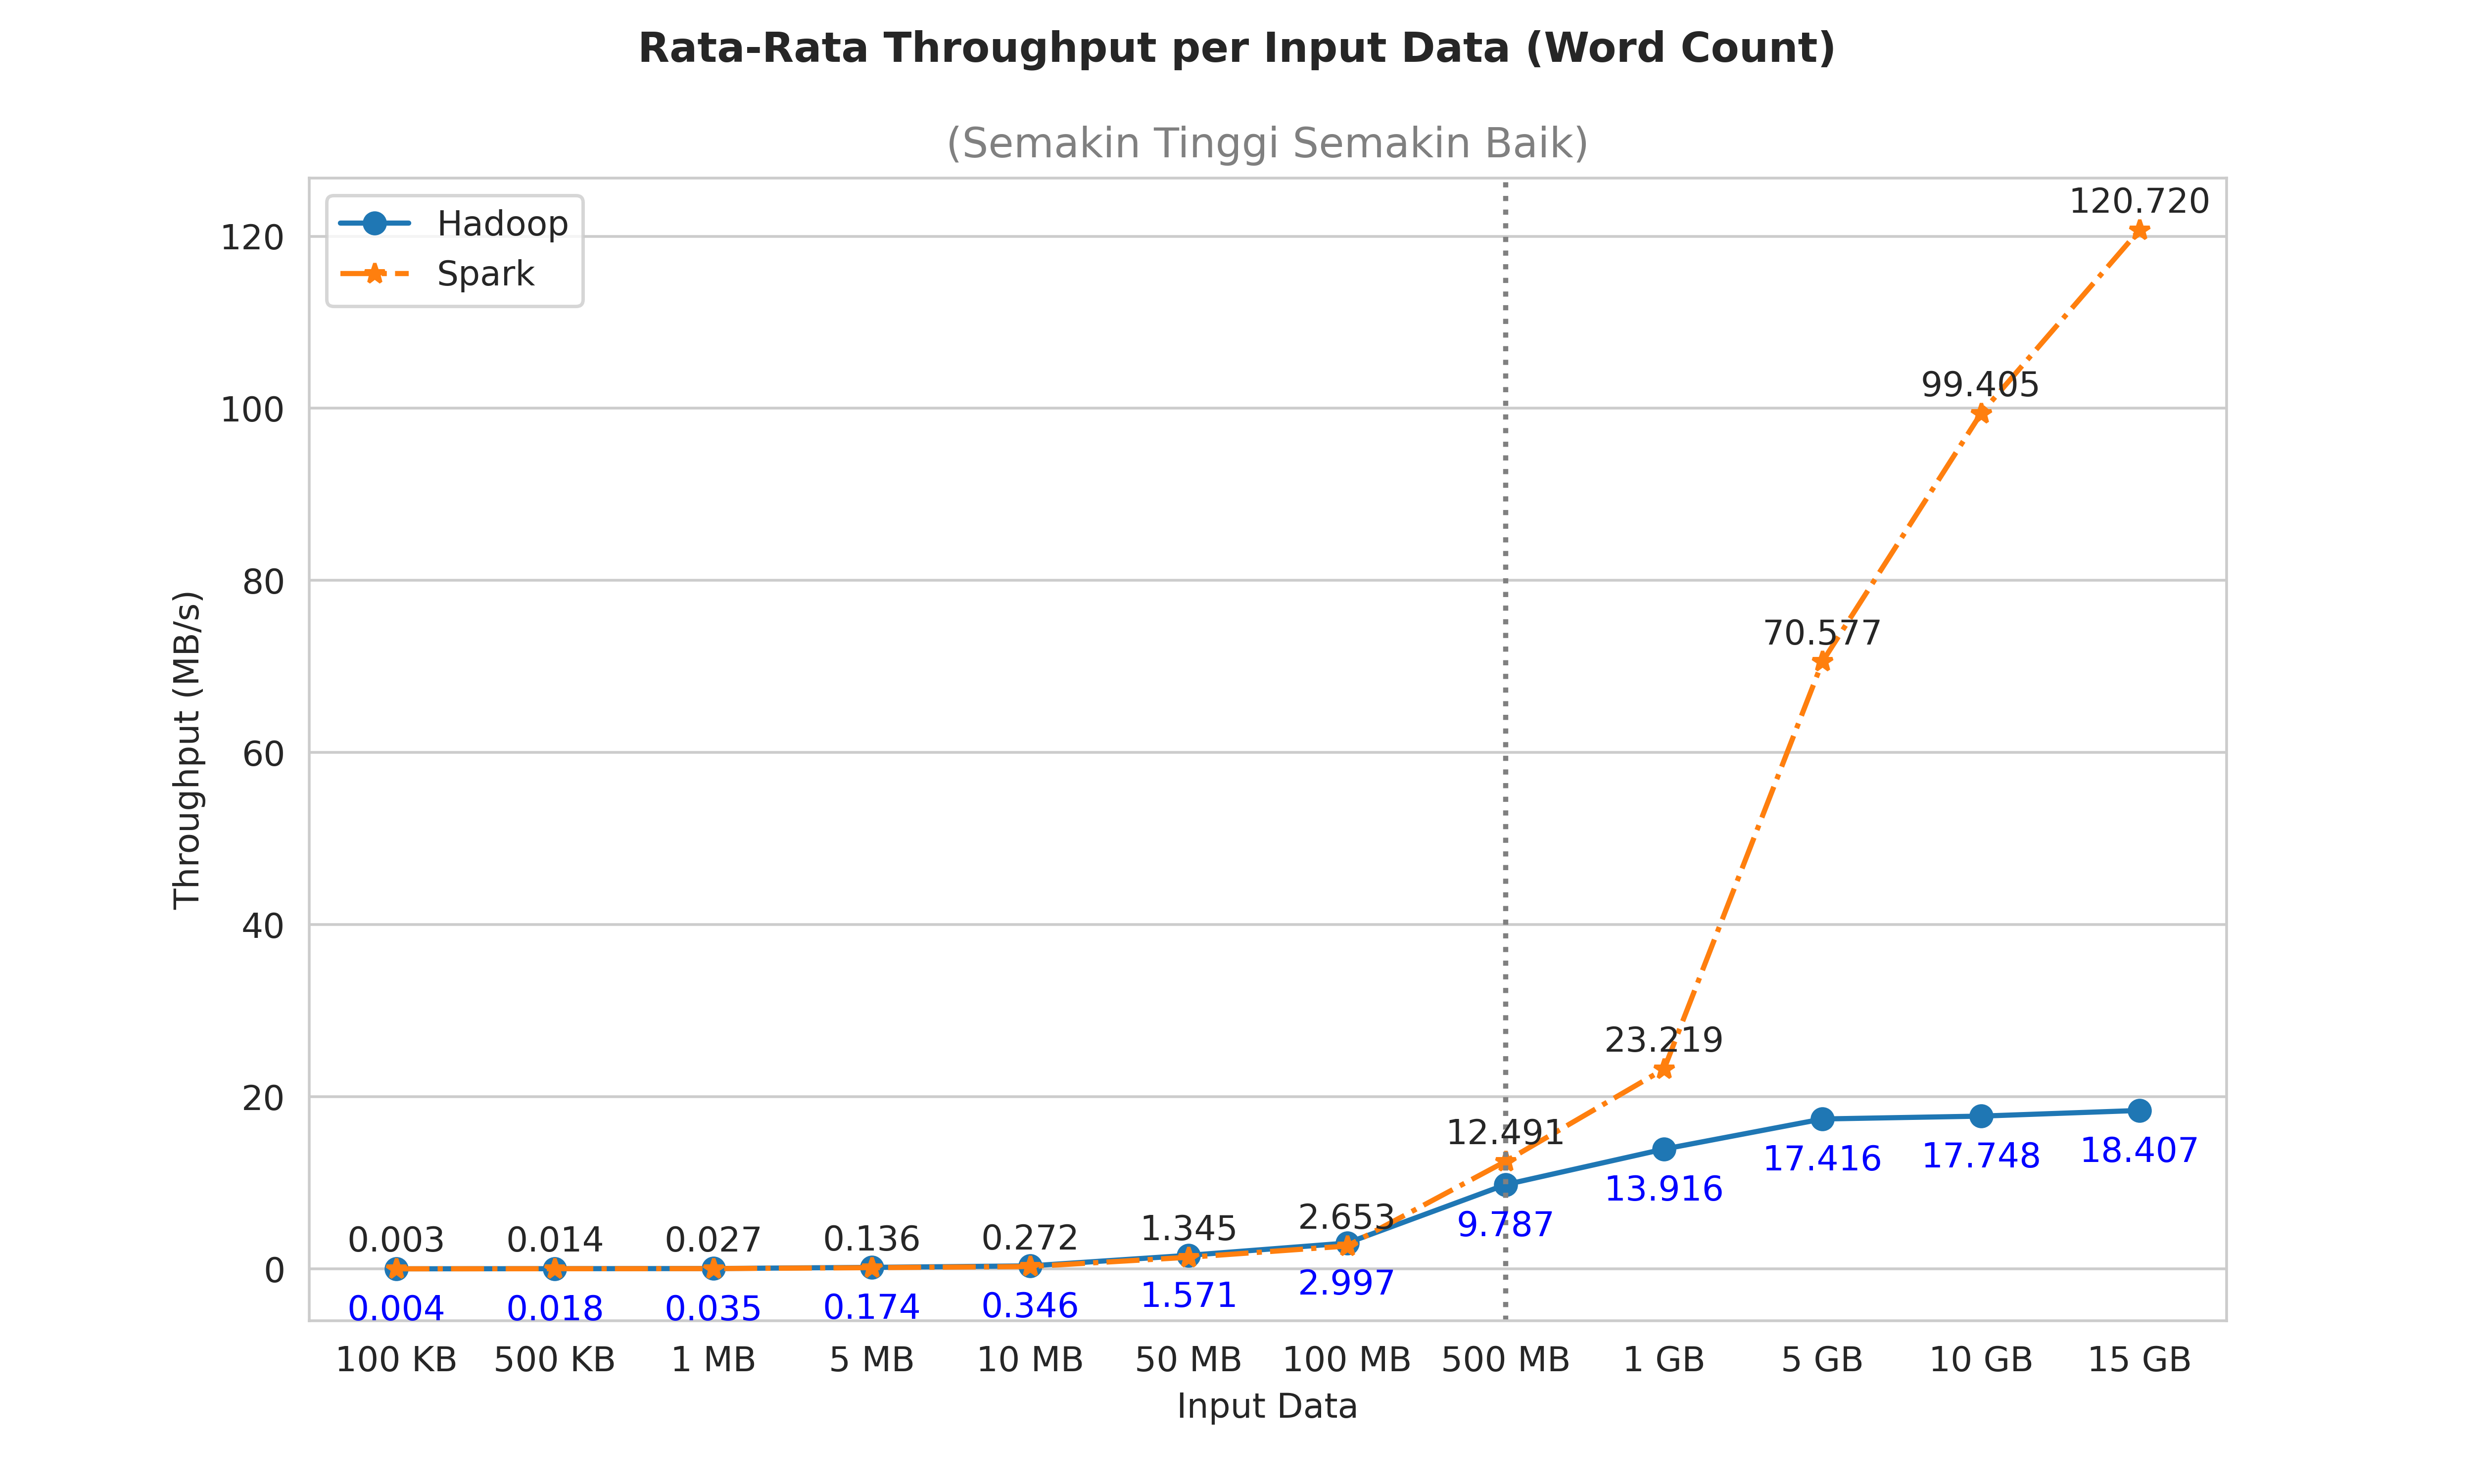
\includegraphics[width=1\textwidth]{figures/ch04/2-mean-throughput-wordcount.png}
    \caption{Rata-rata \textit{Throughput (Word Count)}}
    \label{fig:mean-throughput-wordcount}
\end{figure}

\subsection{Rate of Change}

\begin{figure}[h]
    \centering
    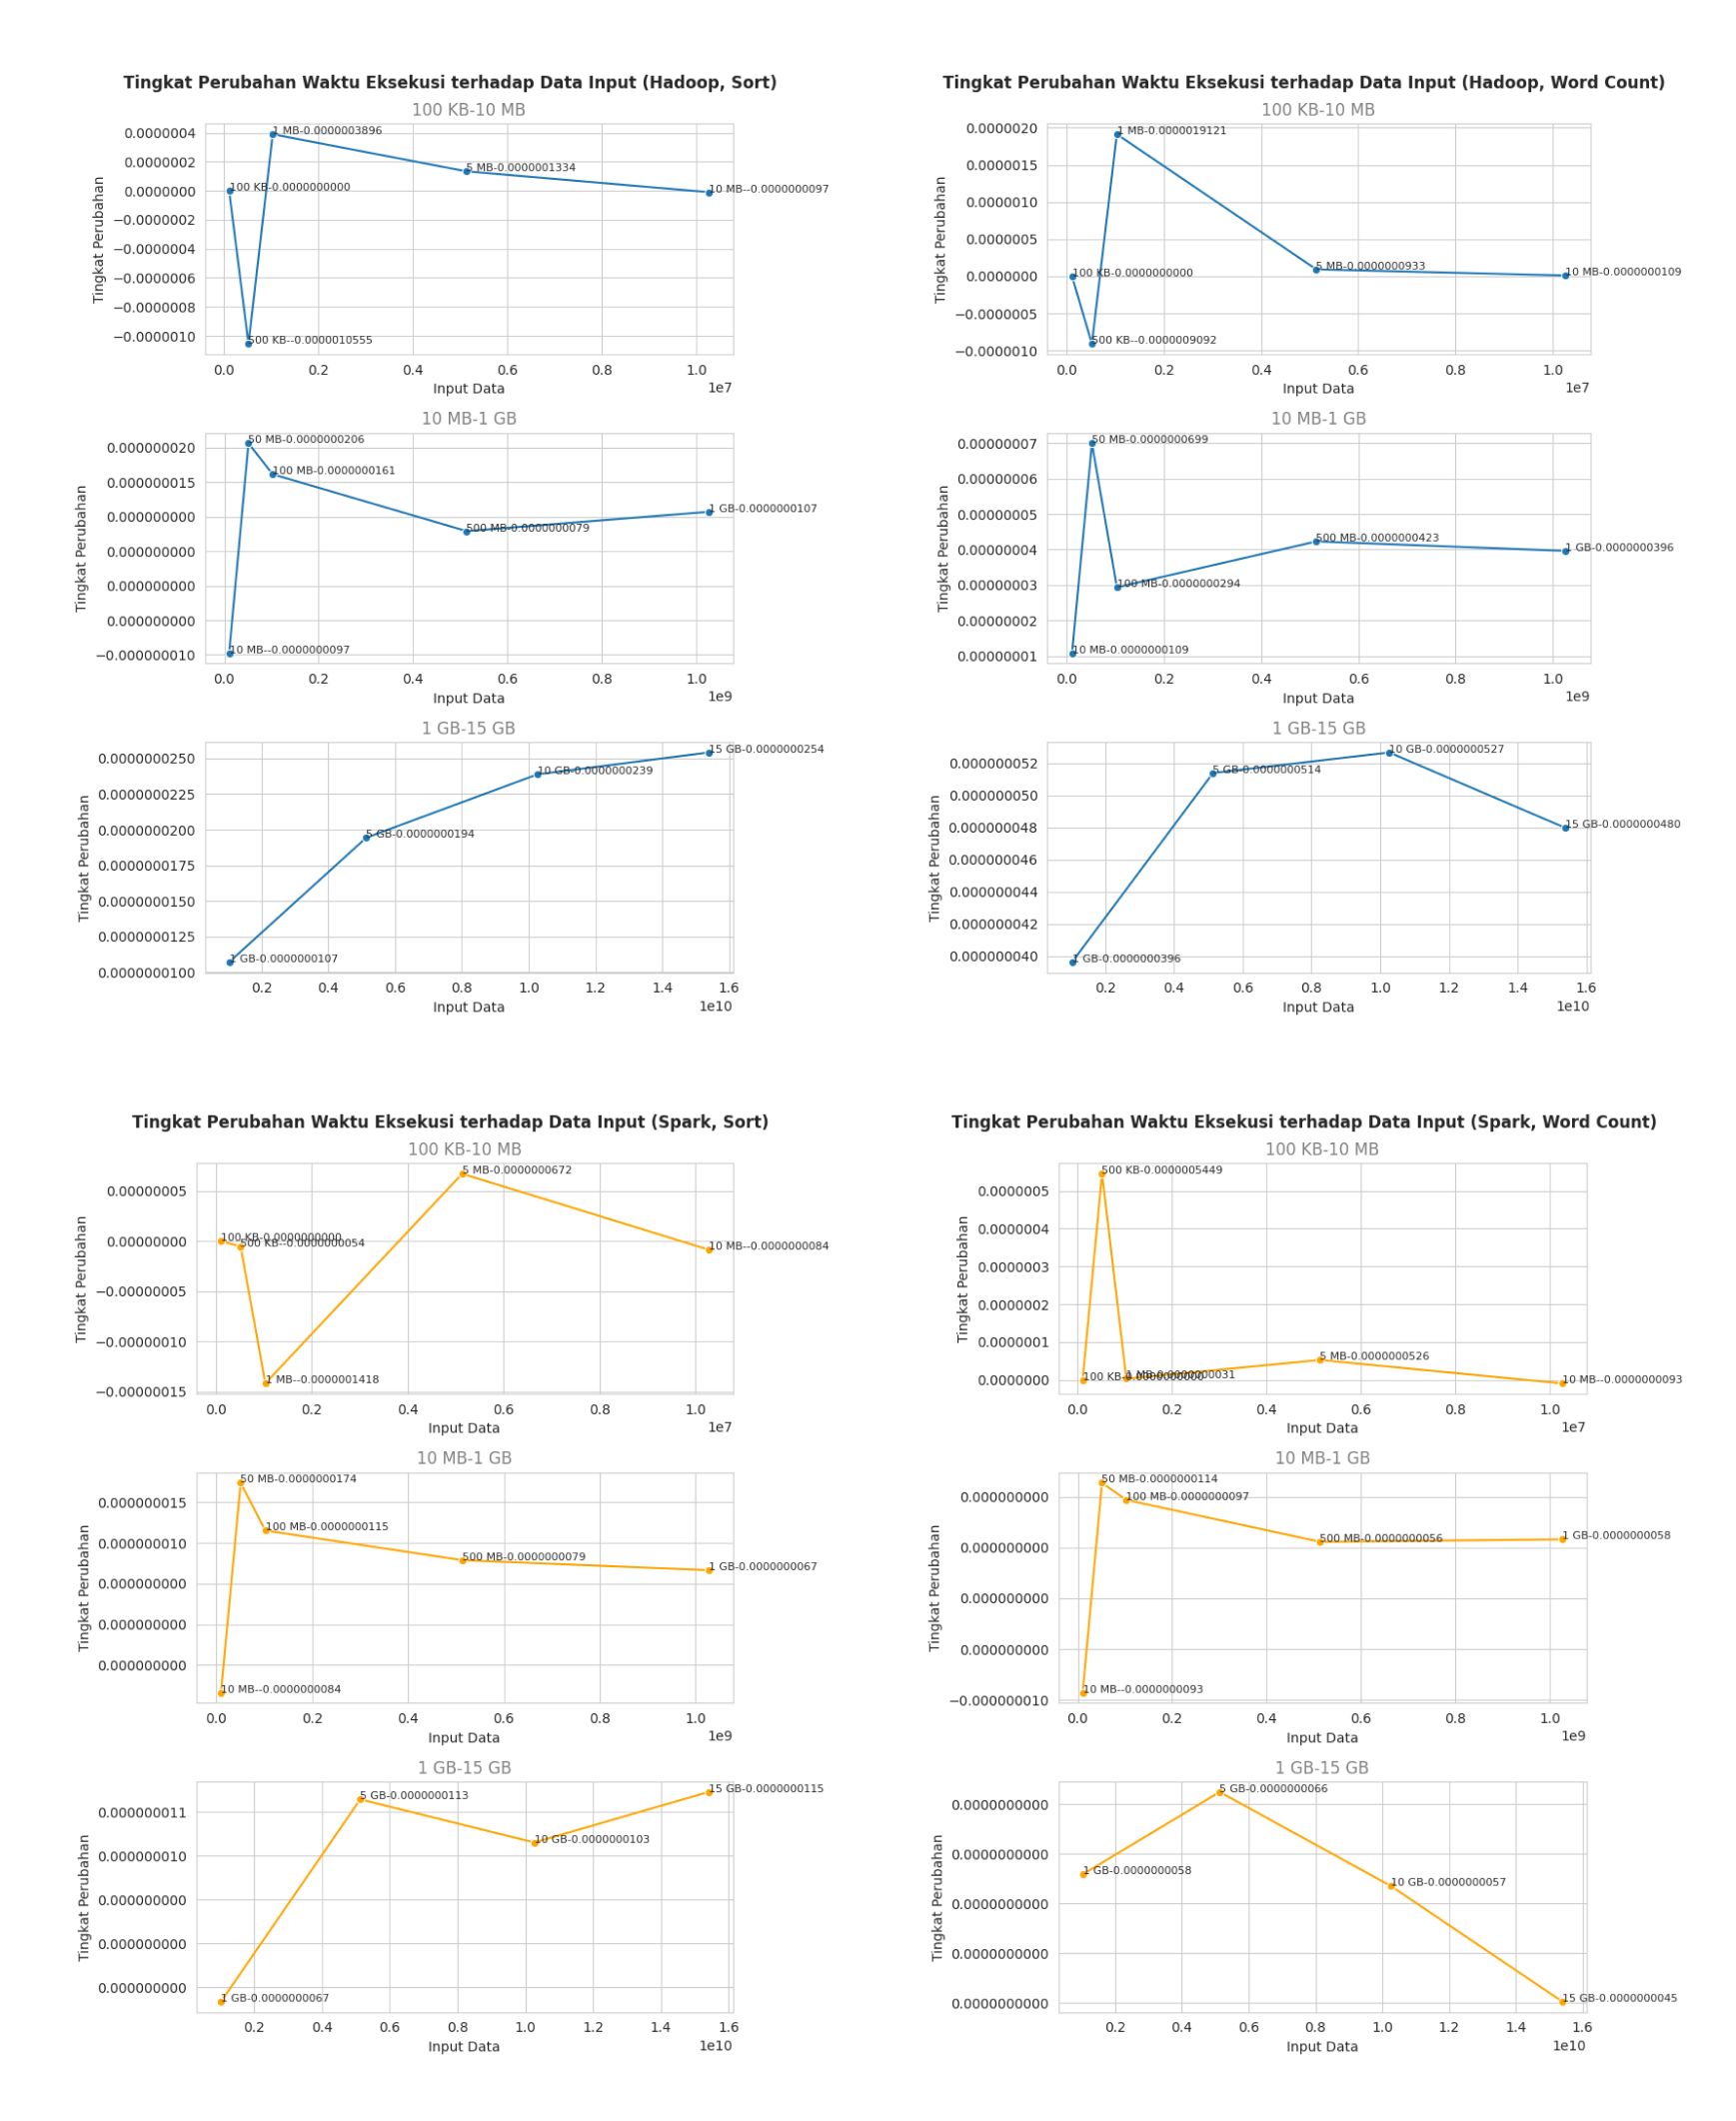
\includegraphics[width=1.1\textwidth]{figures/ch04/3-grup-dur.png}
    \caption{dur}
    \label{fig:3-grup-dur}
\end{figure}

\begin{figure}[h]
    \centering
    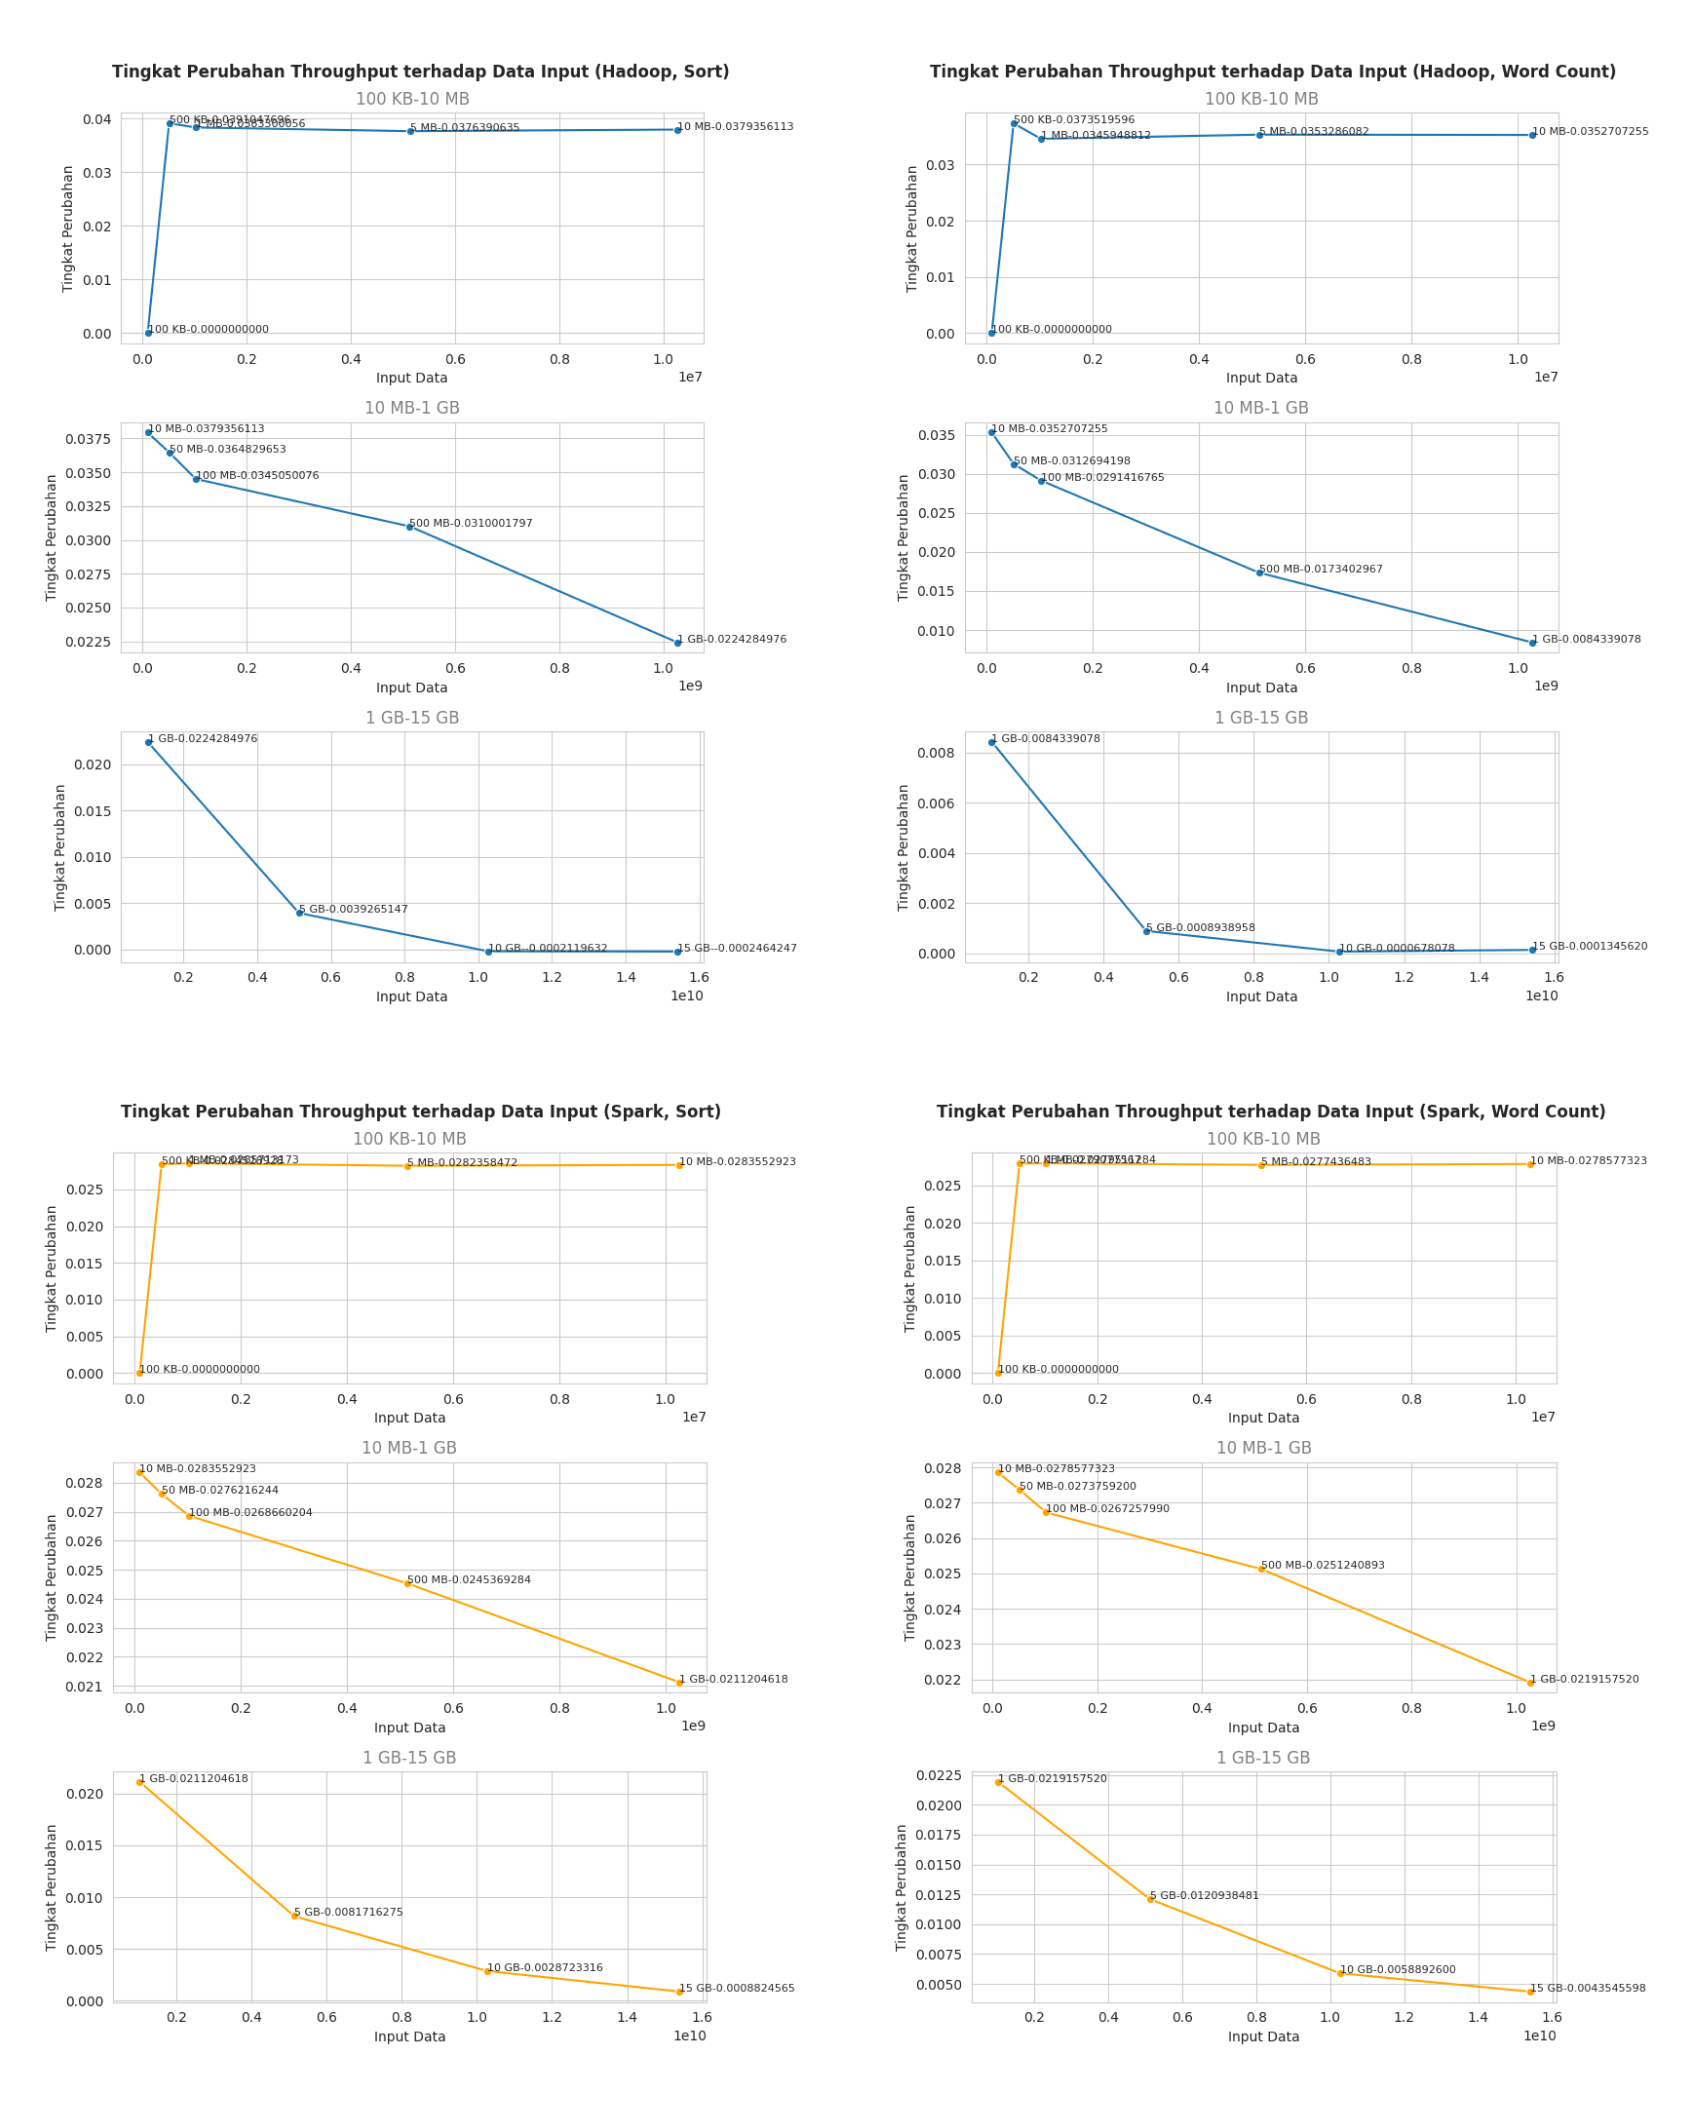
\includegraphics[width=1.1\textwidth]{figures/ch04/3-grup-th.png}
    \caption{th}
    \label{fig:3-grup-th}
\end{figure}

\begin{figure}[h]
    \centering
    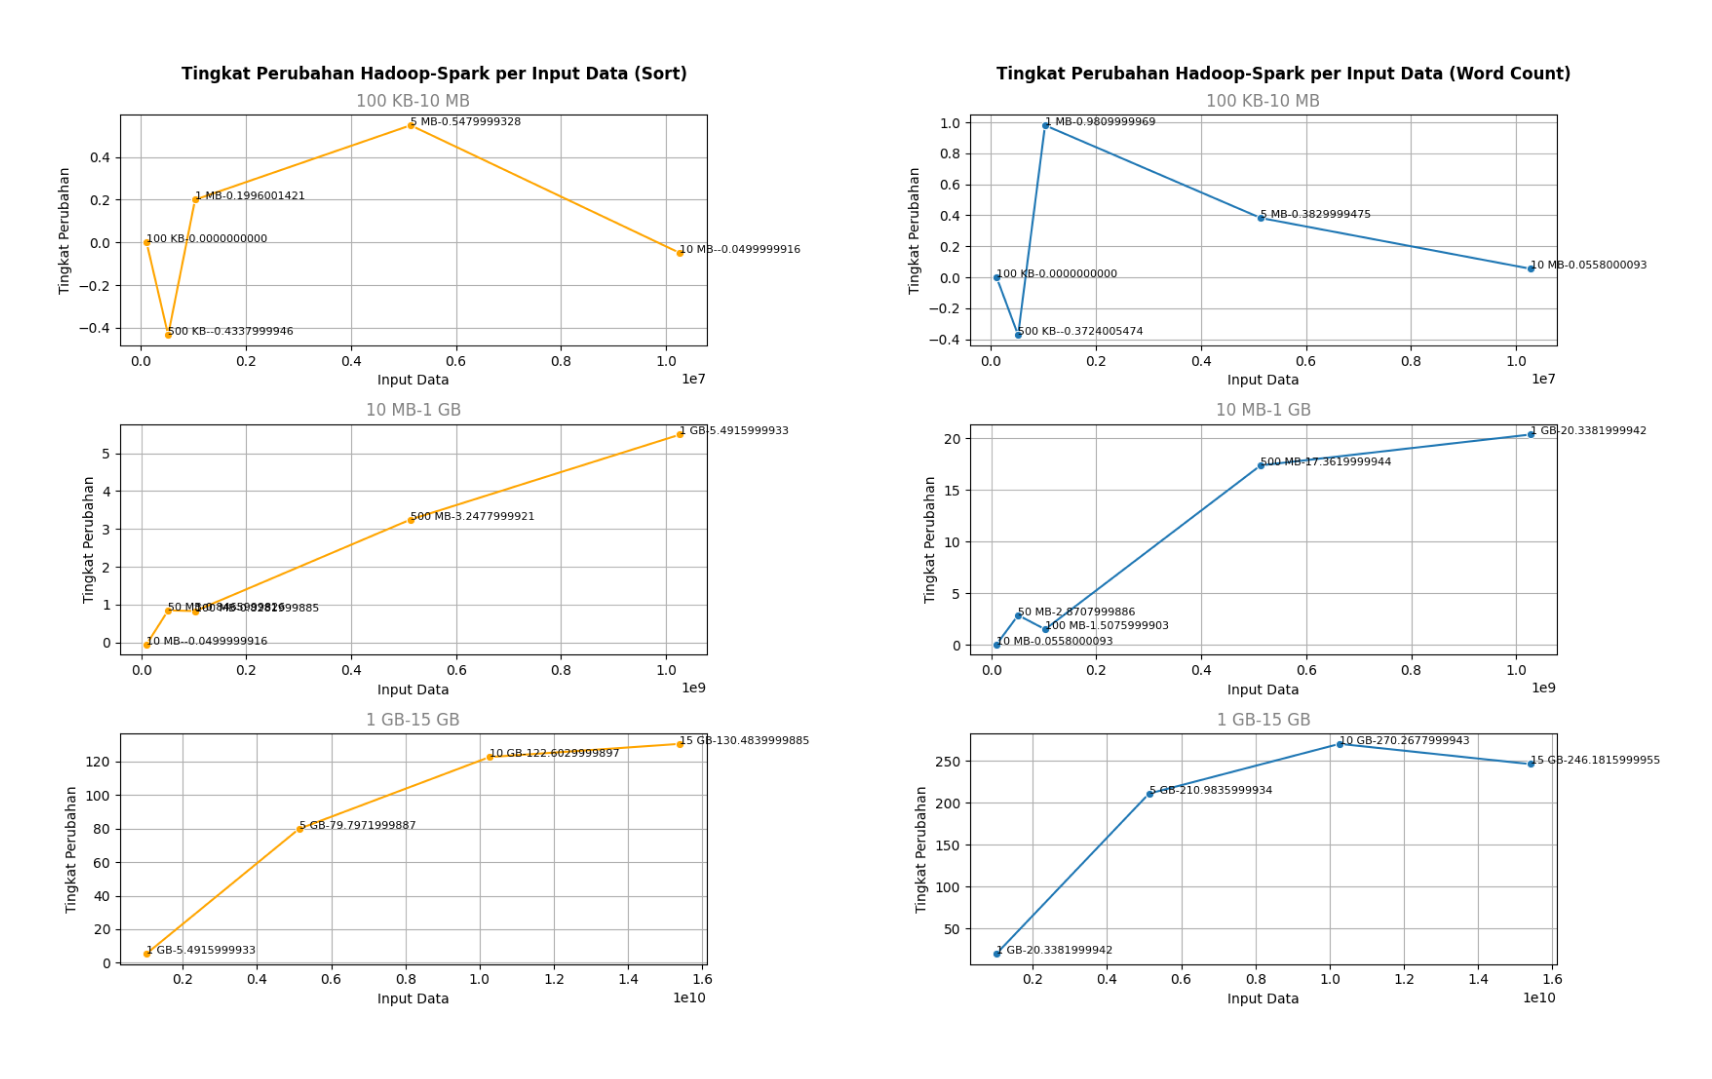
\includegraphics[width=1.1\textwidth]{figures/ch04/3-grup-hadoop-spark.png}
    \caption{hadoop-spark}
    \label{fig:3-grup-hadoop-spark}
\end{figure}


\subsection{Penggunaan CPU}
Gambar \ref{fig:4-penggunaan-cpu-all-sort} dan \ref{fig:4-penggunaan-cpu-all-wordcount} menunjukkan pola penggunaan CPU oleh Hadoop dan Spark untuk tugas sorting dan word count pada berbagai ukuran data. Sumbu x mewakili waktu dalam detik, sedangkan sumbu y mewakili persentase penggunaan CPU. Setiap baris grafik menunjukkan ukuran data yang berbeda, mulai dari 100 KB hingga 15 GB.

Pada kedua tugas, terlihat bahwa Spark cenderung menunjukkan pola penggunaan CPU yang lebih stabil dan konsisten dibandingkan dengan Hadoop. Penggunaan CPU Spark umumnya lebih tinggi dan merata di sepanjang waktu eksekusi, mengindikasikan pemanfaatan sumber daya yang lebih efisien dan pemrosesan paralel yang lebih optimal. Di sisi lain, penggunaan CPU Hadoop cenderung lebih fluktuatif, dengan periode lonjakan dan penurunan yang signifikan. 

Pada tugas sorting (Gambar \ref{fig:4-penggunaan-cpu-all-sort}), perbedaan pola penggunaan CPU antara Hadoop dan Spark semakin terlihat pada ukuran data yang lebih besar. Spark mempertahankan penggunaan CPU yang tinggi dan stabil, sementara Hadoop menunjukkan fluktuasi yang lebih besar dan cenderung menurun pada akhir eksekusi. Hal ini menunjukkan bahwa Spark lebih mampu menangani data besar secara efisien dan konsisten. 

Pada tugas word count (Gambar \ref{fig:4-penggunaan-cpu-all-wordcount}), perbedaan pola penggunaan CPU tidak sejelas pada tugas sorting. Namun, Spark tetap menunjukkan penggunaan CPU yang lebih stabil dan tinggi secara keseluruhan dibandingkan dengan Hadoop. 

\begin{figure}[h]
    \centering
    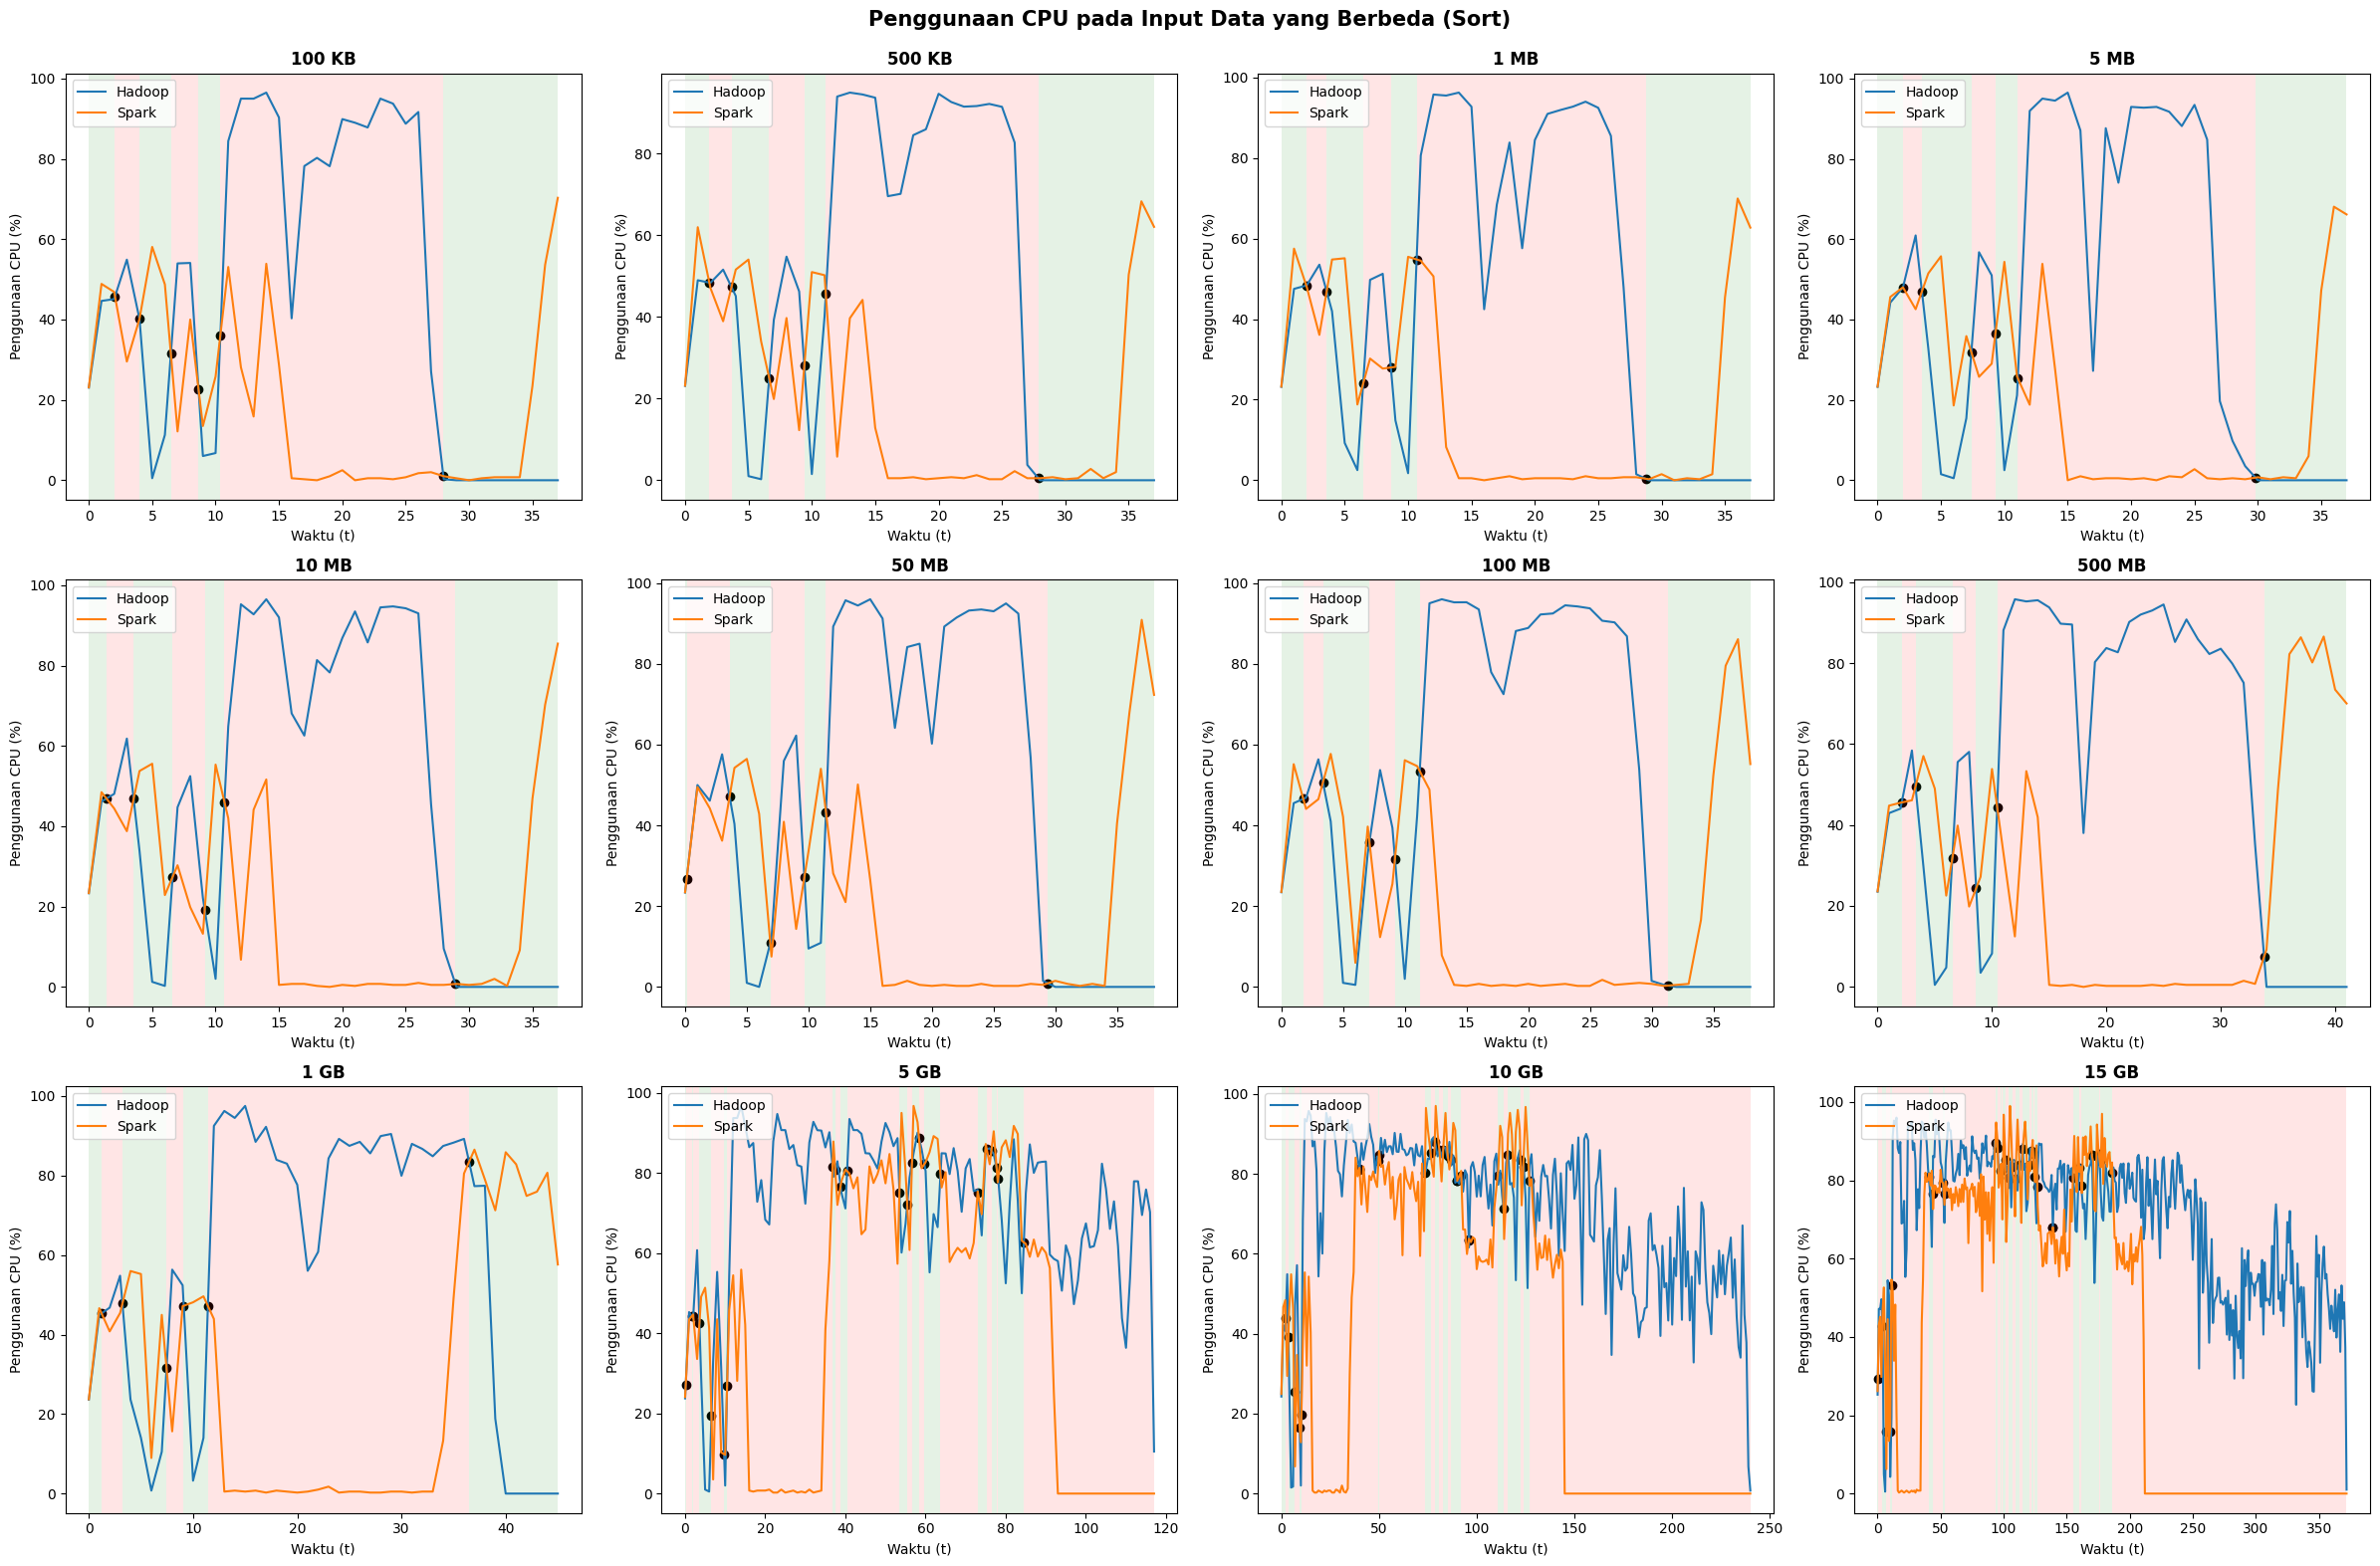
\includegraphics[width=1\textwidth]{figures/ch04/4-penggunaan-cpu-all-sort.png}
    \caption{Penggunaan CPU (Sort)}
    \label{fig:4-penggunaan-cpu-all-sort}
\end{figure}

\begin{figure}[h]
    \centering
    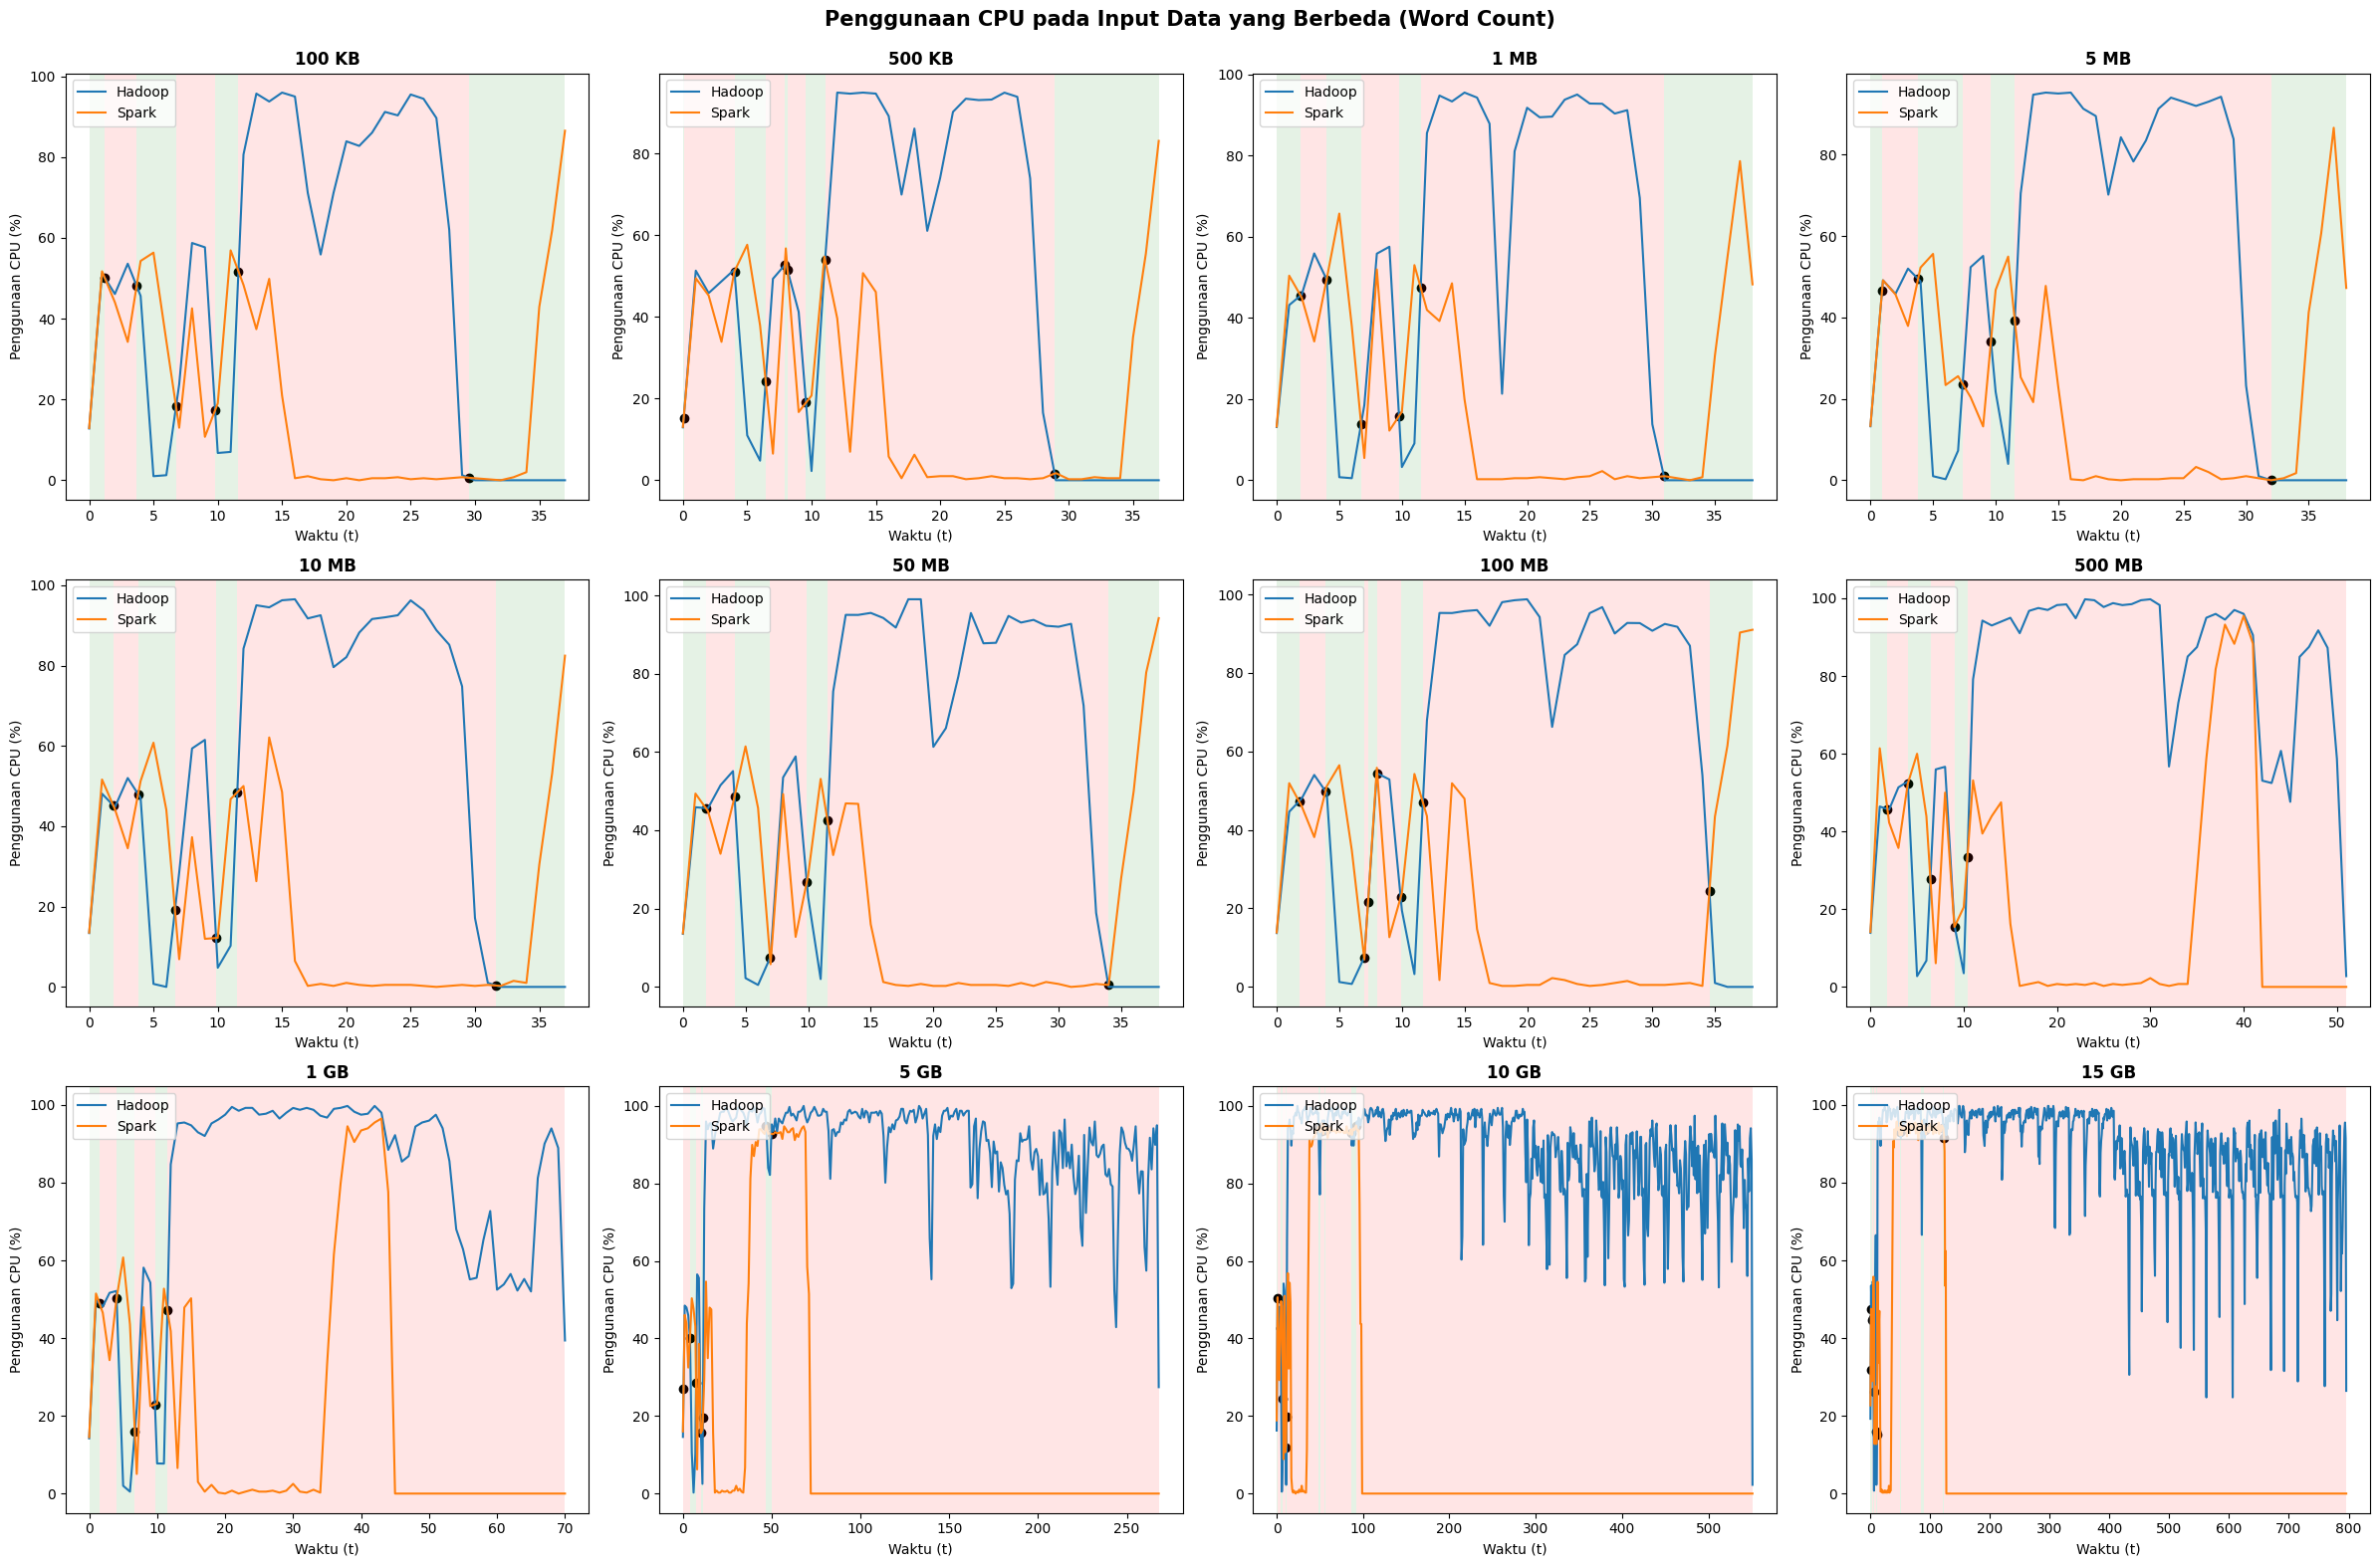
\includegraphics[width=1\textwidth]{figures/ch04/4-penggunaan-cpu-all-wordcount.png}
    \caption{Penggunaan CPU (Word Count)}
    \label{fig:4-penggunaan-cpu-all-wordcount}
\end{figure}

Gambar \ref{fig:4-state-sort} dan \ref{fig:4-state-wordcount} menyajikan bar chart yang menggambarkan perbandingan persentase state $U_s$ (user) antara Hadoop dan Spark untuk tugas sorting dan word count pada berbagai ukuran data dan skenario. State $U_s$ merepresentasikan waktu CPU yang dihabiskan dalam mode user, yang menunjukkan waktu yang dihabiskan untuk menjalankan kode aplikasi. 

Pada kedua tugas, Spark secara konsisten menunjukkan persentase state $U_s$ yang lebih tinggi dibandingkan dengan Hadoop. Hal ini menunjukkan bahwa Spark lebih efisien dalam memanfaatkan waktu CPU untuk menjalankan kode aplikasi, sementara Hadoop menghabiskan lebih banyak waktu dalam state lain, seperti state sistem ($S_s$) atau state idle ($I_s$). 

\begin{figure}[h]
    \centering
    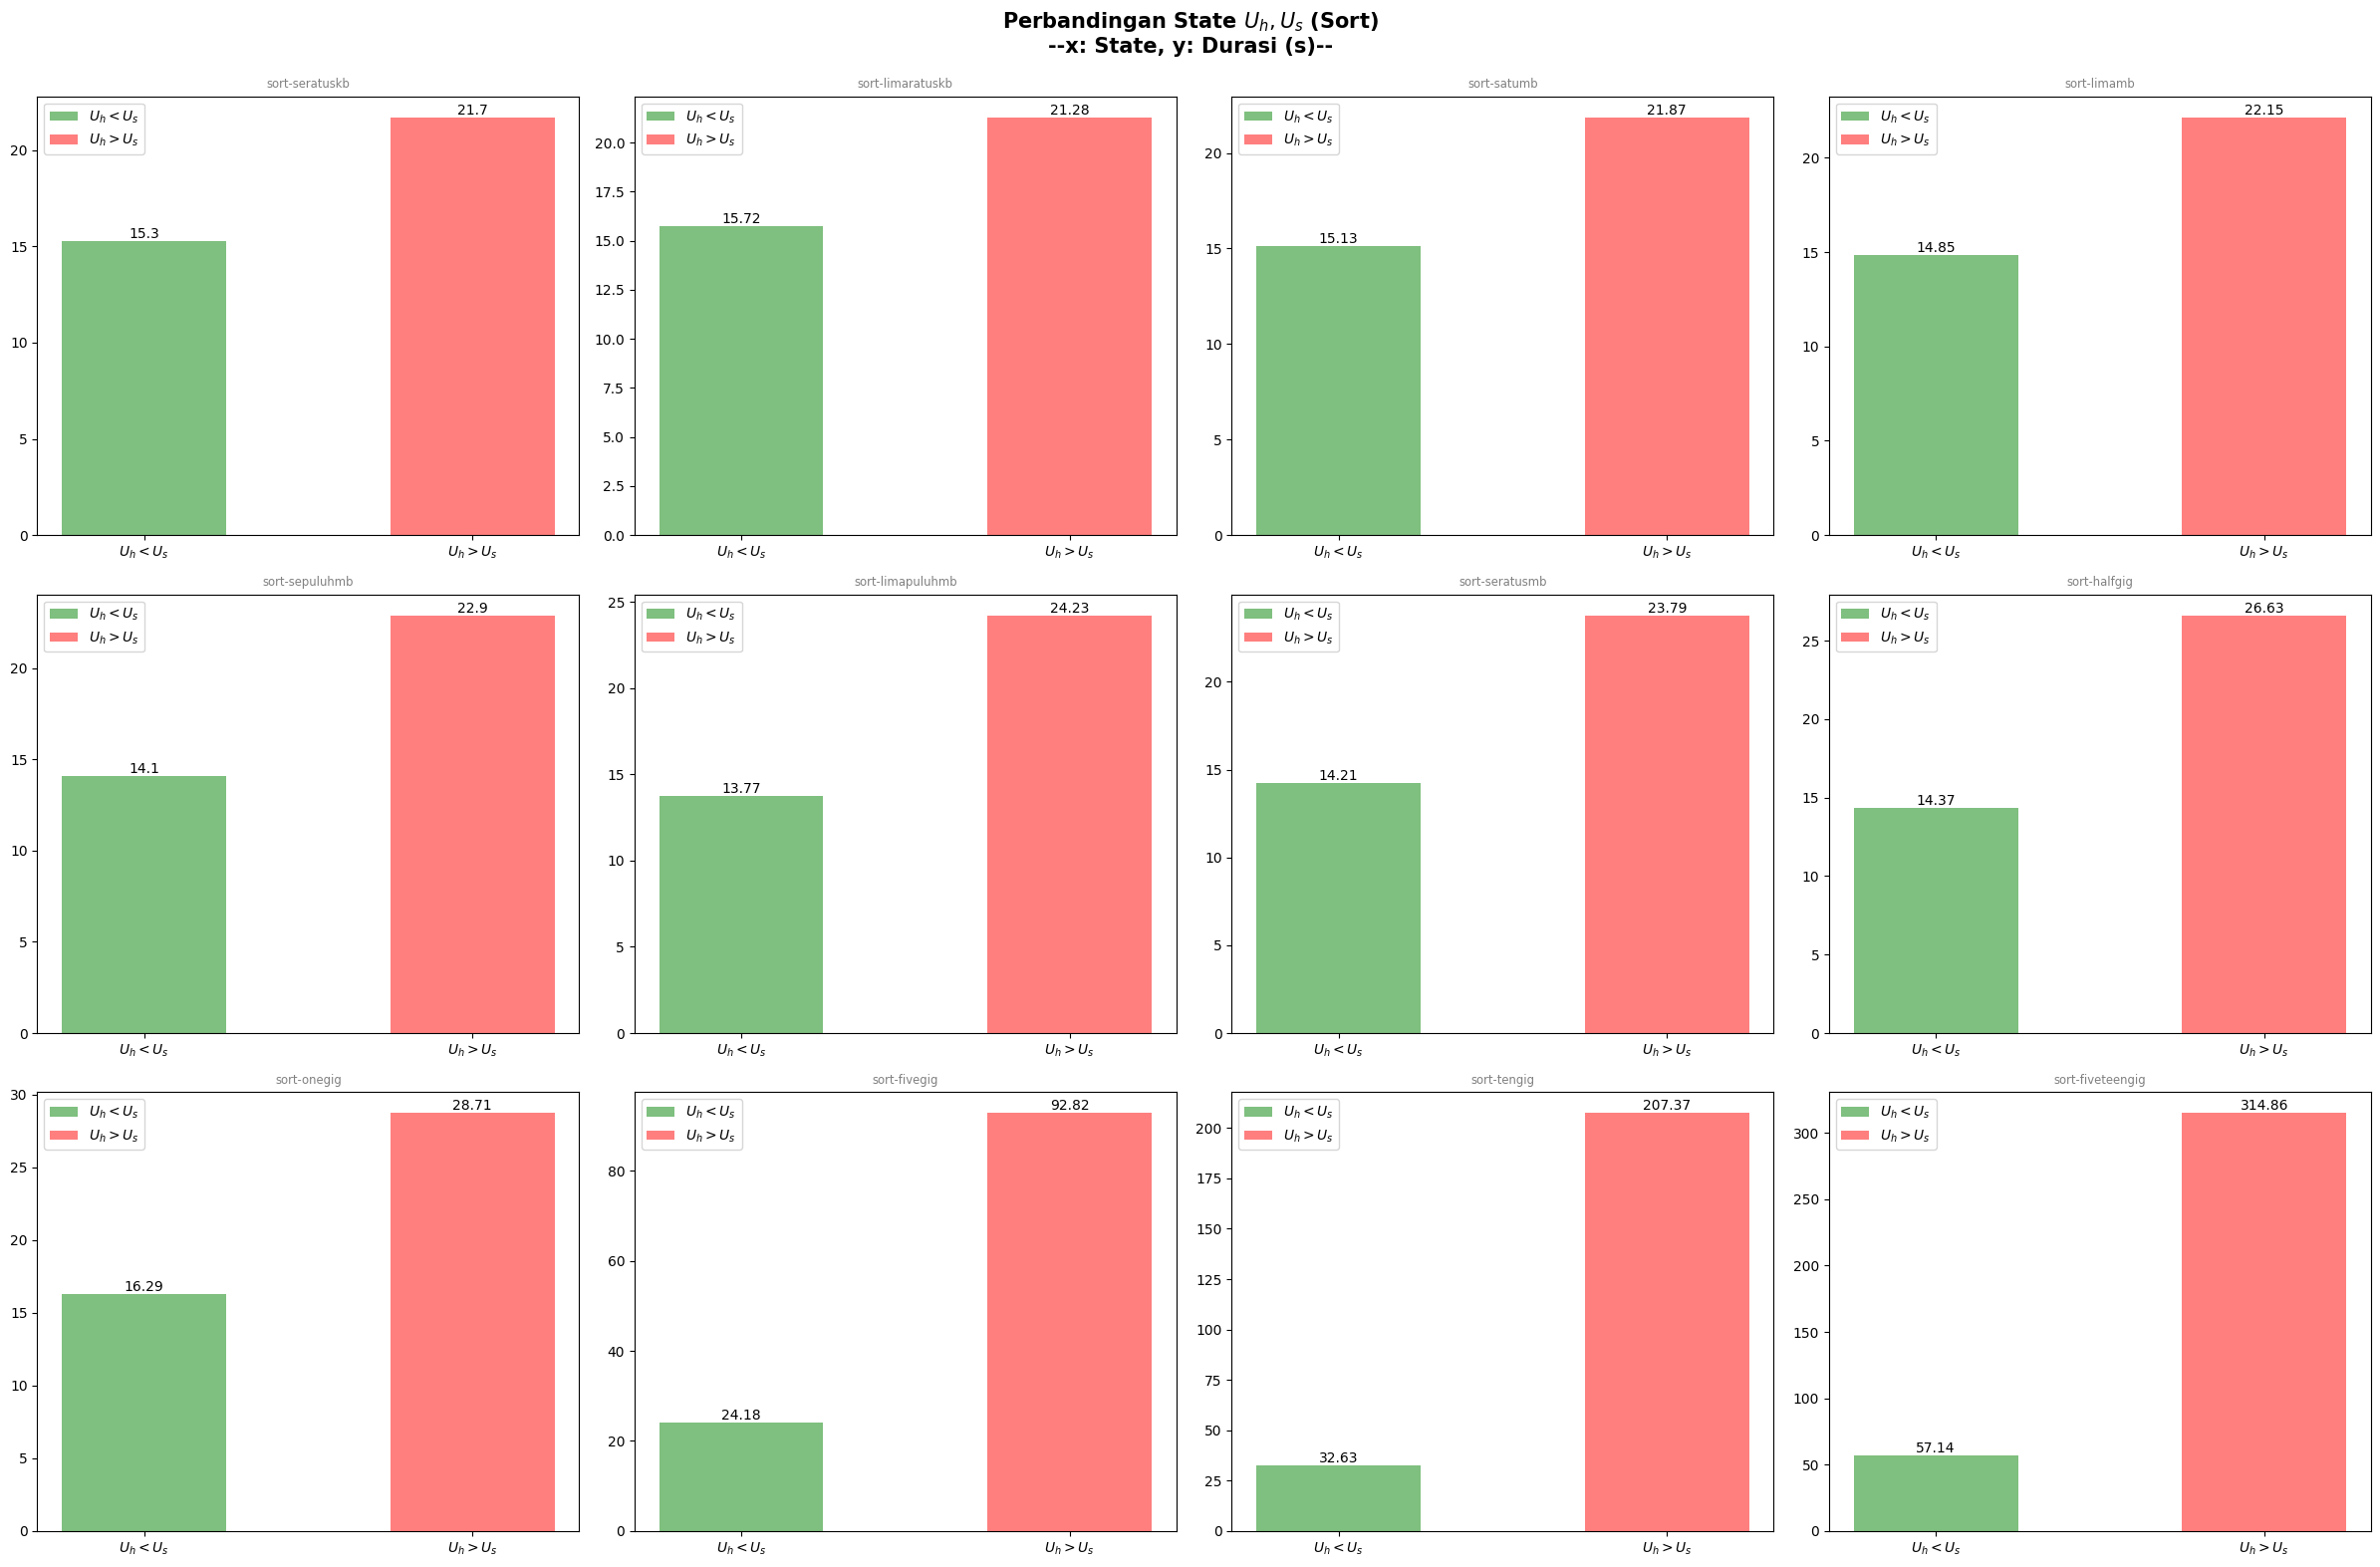
\includegraphics[width=1\textwidth]{figures/ch04/4-state-sort.png}
    \caption{State (Sort)}
    \label{fig:4-state-sort}
\end{figure}

\begin{figure}[h]
    \centering
    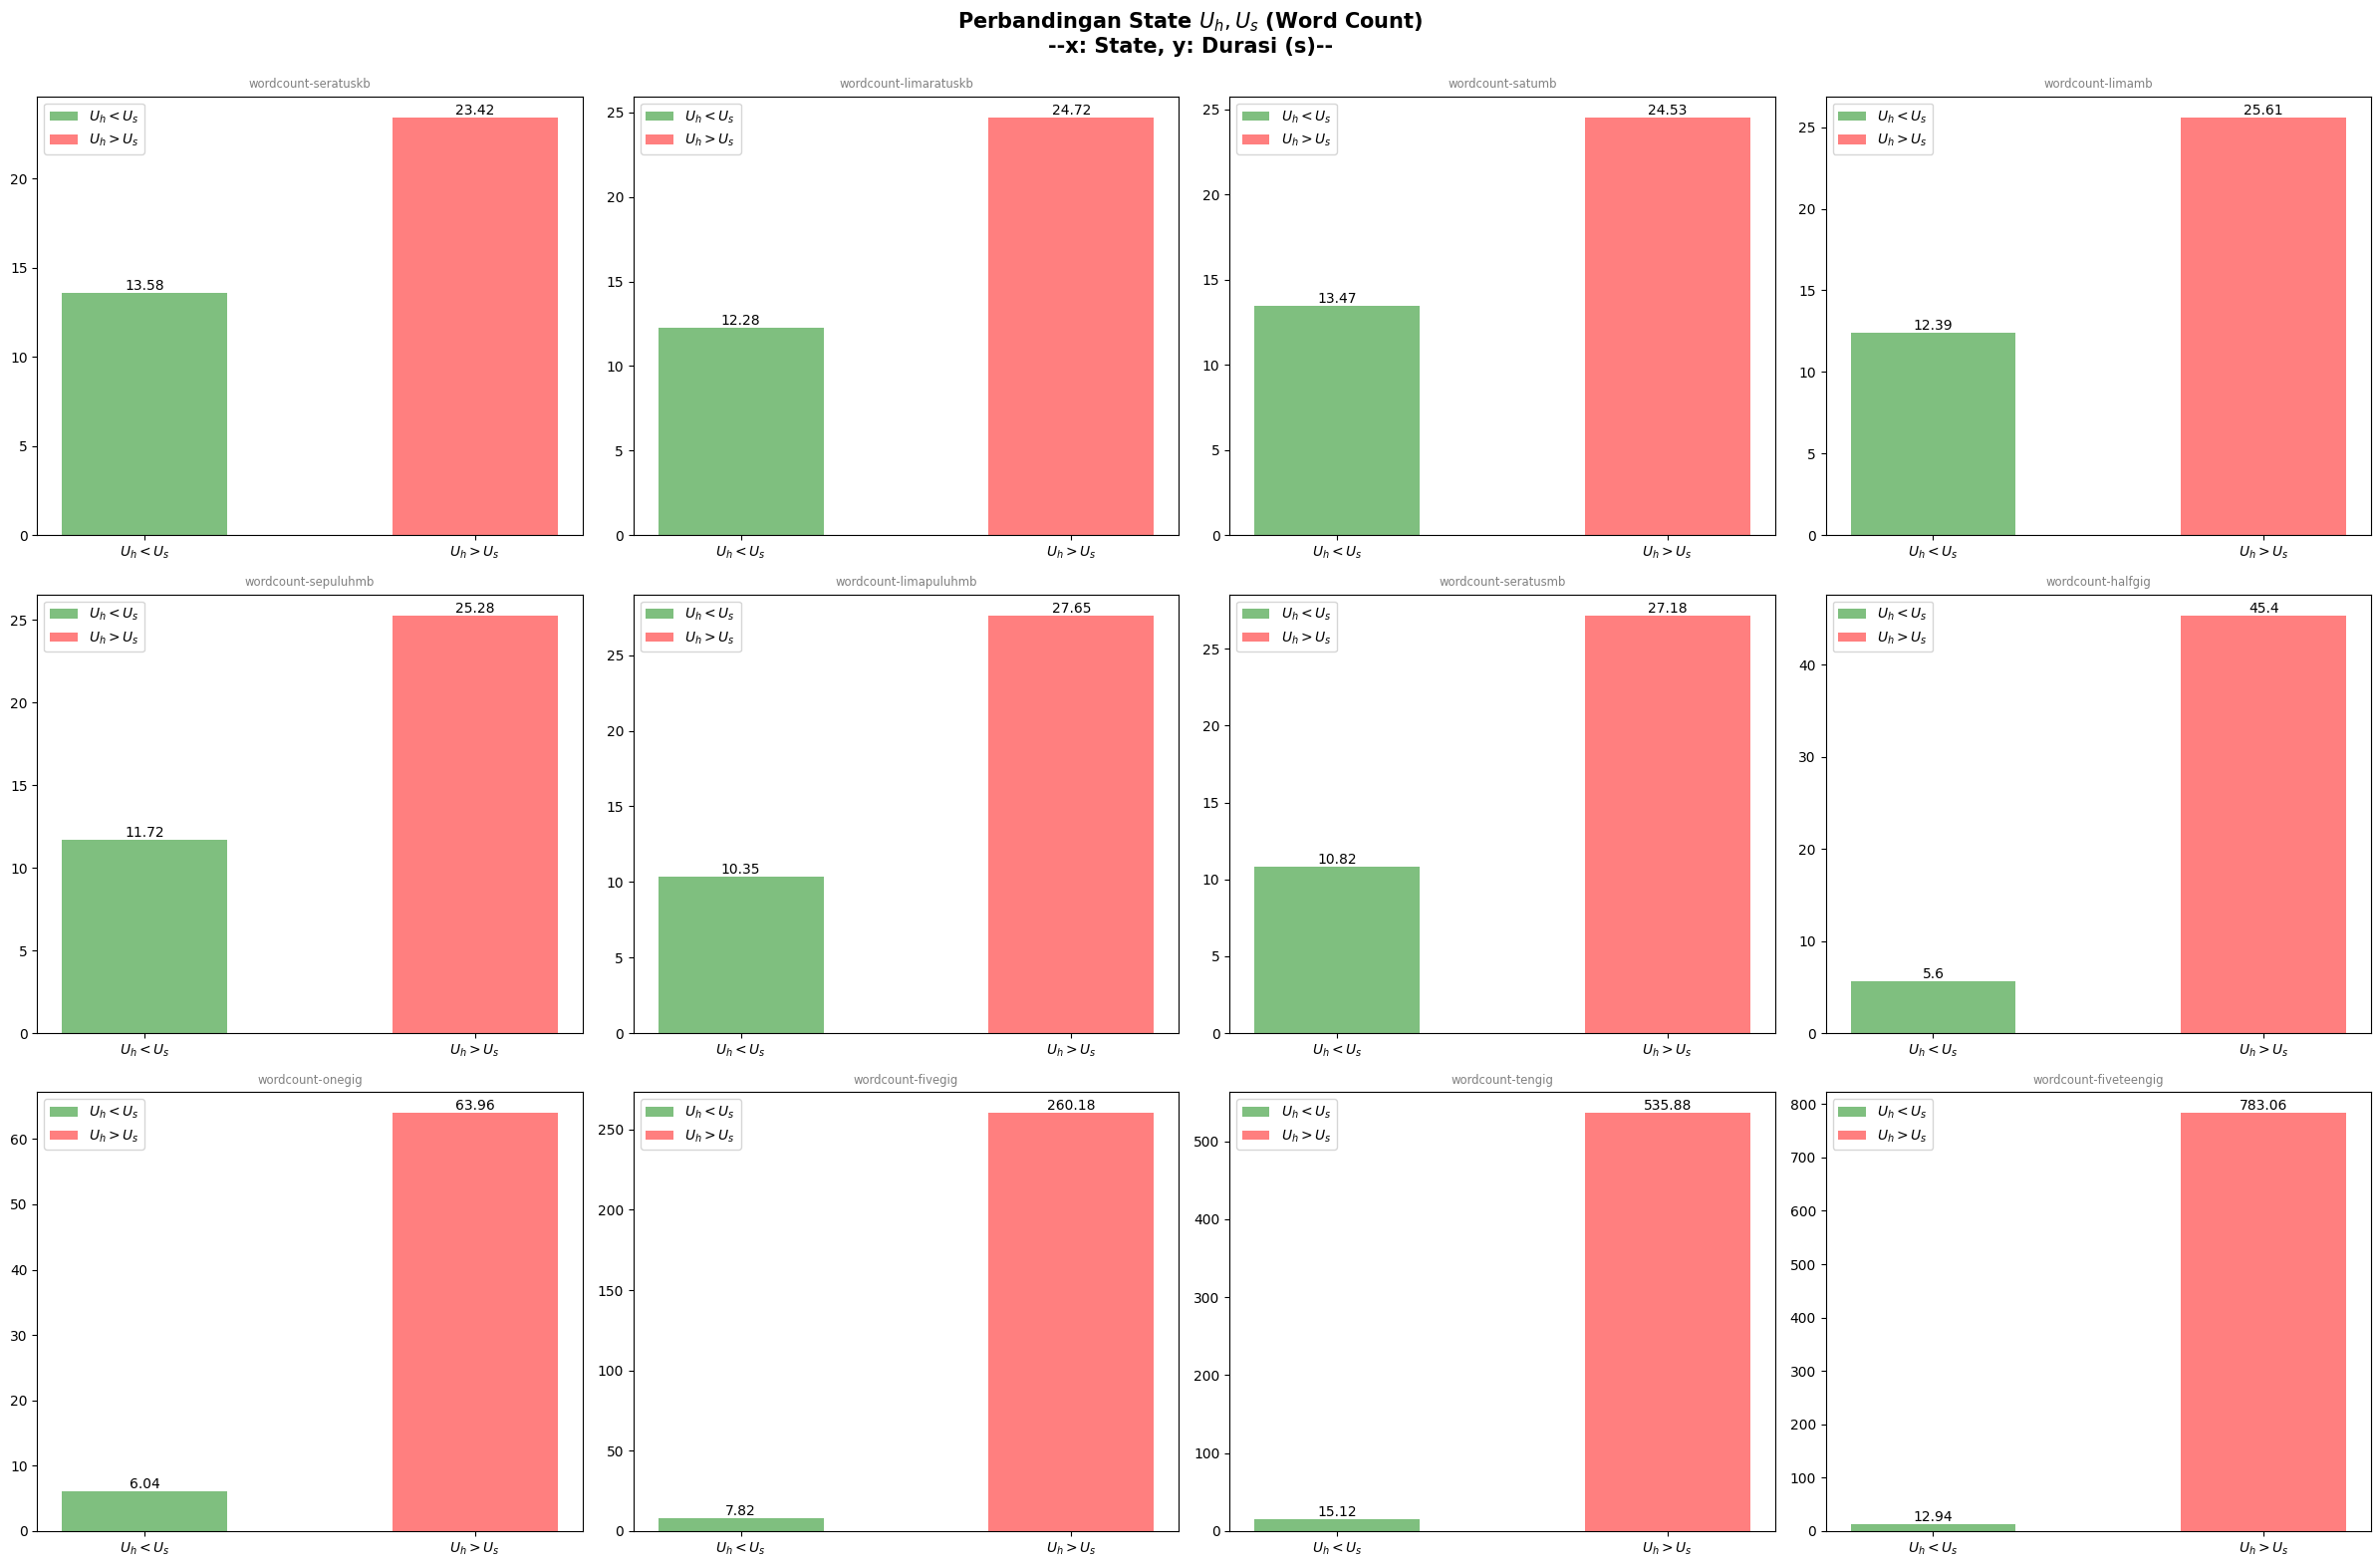
\includegraphics[width=1\textwidth]{figures/ch04/4-state-wordcount.png}
    \caption{State (Word Count)}
    \label{fig:4-state-wordcount}
\end{figure}

Pada tugas sorting (Gambar \ref{fig:4-state-sort}), perbedaan persentase state $U_s$ antara Spark dan Hadoop semakin terlihat pada ukuran data yang lebih besar. Hal ini menunjukkan bahwa Spark lebih mampu memaksimalkan penggunaan CPU untuk tugas komputasi intensif seperti sorting, terutama saat menangani data dalam jumlah besar.

Pada tugas word count (Gambar \ref{fig:4-state-wordcount}), meskipun Spark masih menunjukkan persentase state $U_s$ yang lebih tinggi, perbedaannya tidak sejelas pada tugas sorting. Hal ini mungkin karena tugas word count tidak seintensif sorting secara komputasi. 

\subsection{Utilisasi Sistem}
Gambar \ref{fig:utilisasi-sort} dan \ref{fig:utilisasi-wordcount} menyajikan informasi pemantauan sistem yang membandingkan penggunaan sumber daya komputasi oleh Hadoop dan Spark selama menjalankan tugas sorting dan word count dengan ukuran data "fiveteengig". Setiap gambar terdiri dari tiga grafik yang menunjukkan penggunaan CPU, Disk I/O, dan memori seiring berjalannya waktu. 

Pada kedua tugas, Spark menunjukkan pola penggunaan CPU yang lebih tinggi dan konsisten dibandingkan dengan Hadoop. Grafik penggunaan CPU Spark menunjukkan garis yang cenderung mendatar di dekat tingkat utilisasi maksimum, mengindikasikan bahwa Spark mampu memaksimalkan pemanfaatan CPU untuk pemrosesan data secara terus-menerus. Di sisi lain, grafik penggunaan CPU Hadoop menunjukkan fluktuasi yang lebih besar, dengan periode lonjakan dan penurunan yang signifikan. Hal ini menunjukkan bahwa Hadoop mengalami periode idle yang lebih lama dan tidak memanfaatkan sumber daya CPU seefisien Spark. 

Hadoop menunjukkan aktivitas Disk I/O yang jauh lebih tinggi dibandingkan dengan Spark, terutama pada tugas sorting (Gambar \ref{fig:utilisasi-sort}). Grafik Disk I/O Hadoop menunjukkan lonjakan aktivitas baca dan tulis yang signifikan sepanjang waktu eksekusi. Hal ini sesuai dengan pendekatan berbasis disk Hadoop yang membutuhkan pembacaan dan penulisan data ke disk secara intensif. Sebaliknya, Spark, dengan arsitektur in-memory, meminimalkan operasi Disk I/O. Grafik Disk I/O Spark menunjukkan aktivitas yang jauh lebih rendah dan stabil, yang berkontribusi pada peningkatan performanya.

Spark menunjukkan penggunaan memori yang lebih tinggi dan stabil dibandingkan dengan Hadoop, terutama pada tugas word count (Gambar \ref{fig:utilisasi-wordcount}). Grafik penggunaan memori Spark menunjukkan garis yang cenderung mendatar pada tingkat utilisasi yang tinggi, menunjukkan bahwa Spark menyimpan data dalam RAM untuk akses yang lebih cepat dan pemrosesan yang efisien. Penggunaan memori Hadoop lebih rendah dan fluktuatif, menunjukkan bahwa Hadoop tidak mema'nfaatkan memori secara optimal. 

Analisis pemantauan sistem menegaskan keunggulan Spark dalam hal efisiensi dan optimasi penggunaan sumber daya komputasi dibandingkan dengan Hadoop. Spark mampu memaksimalkan penggunaan CPU, meminimalkan operasi Disk I/O, dan memanfaatkan memori secara efisien, yang berkontribusi pada performa dan skalabilitas yang lebih baik dalam tugas-tugas pemrosesan data besar.

\subsubsection{Input Data 100 KB}
\begin{figure}[h]
    \centering
    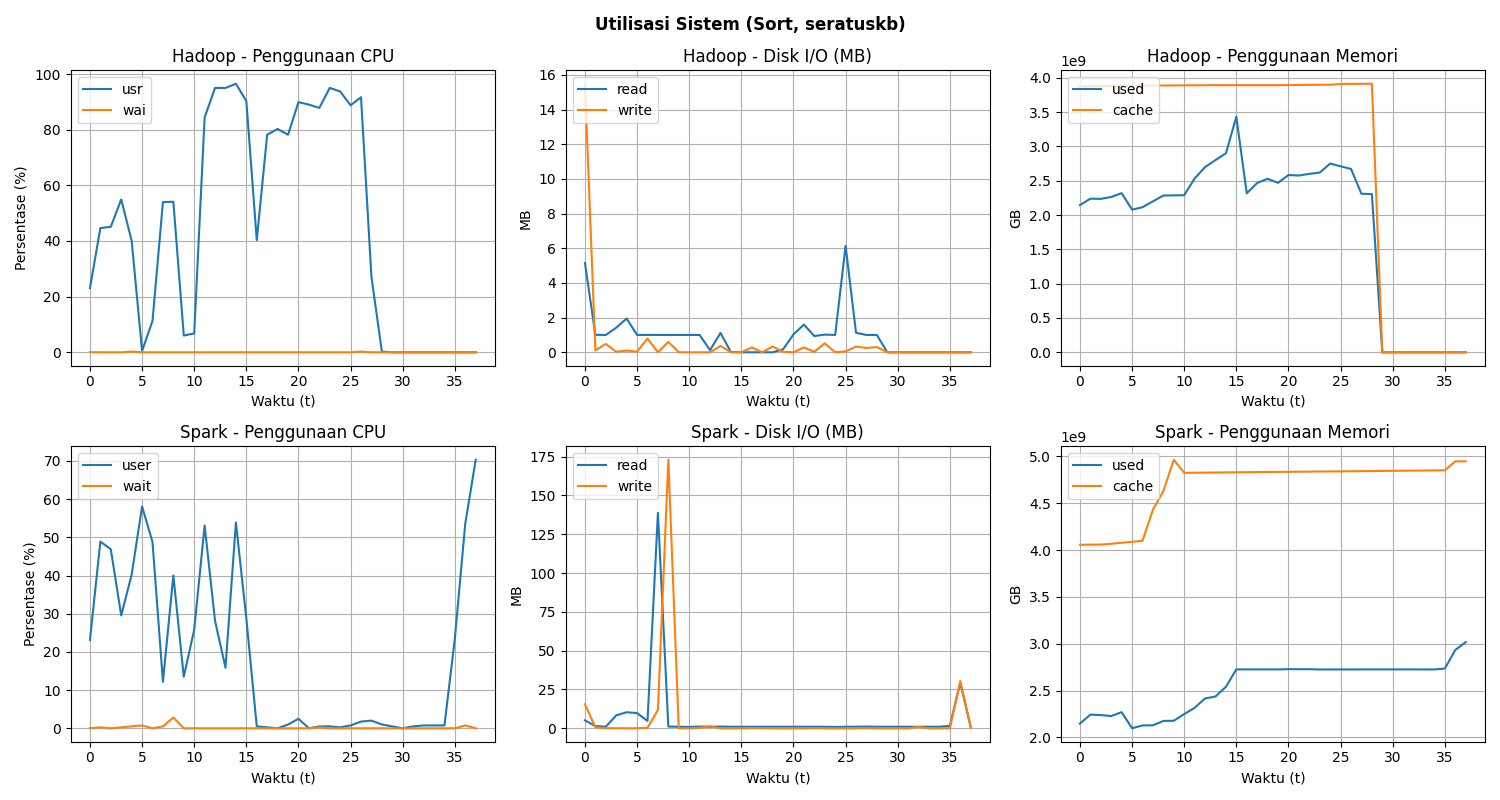
\includegraphics[width=1\textwidth]{figures/ch04/5-util-sistem-sort-seratuskb}
    \caption{Utilisasi Sistem (Sort) pada Input Data 100 KB}
    \label{fig:5-util-sistem-sort-seratuskb}
\end{figure}

\begin{figure}[h]
    \centering
    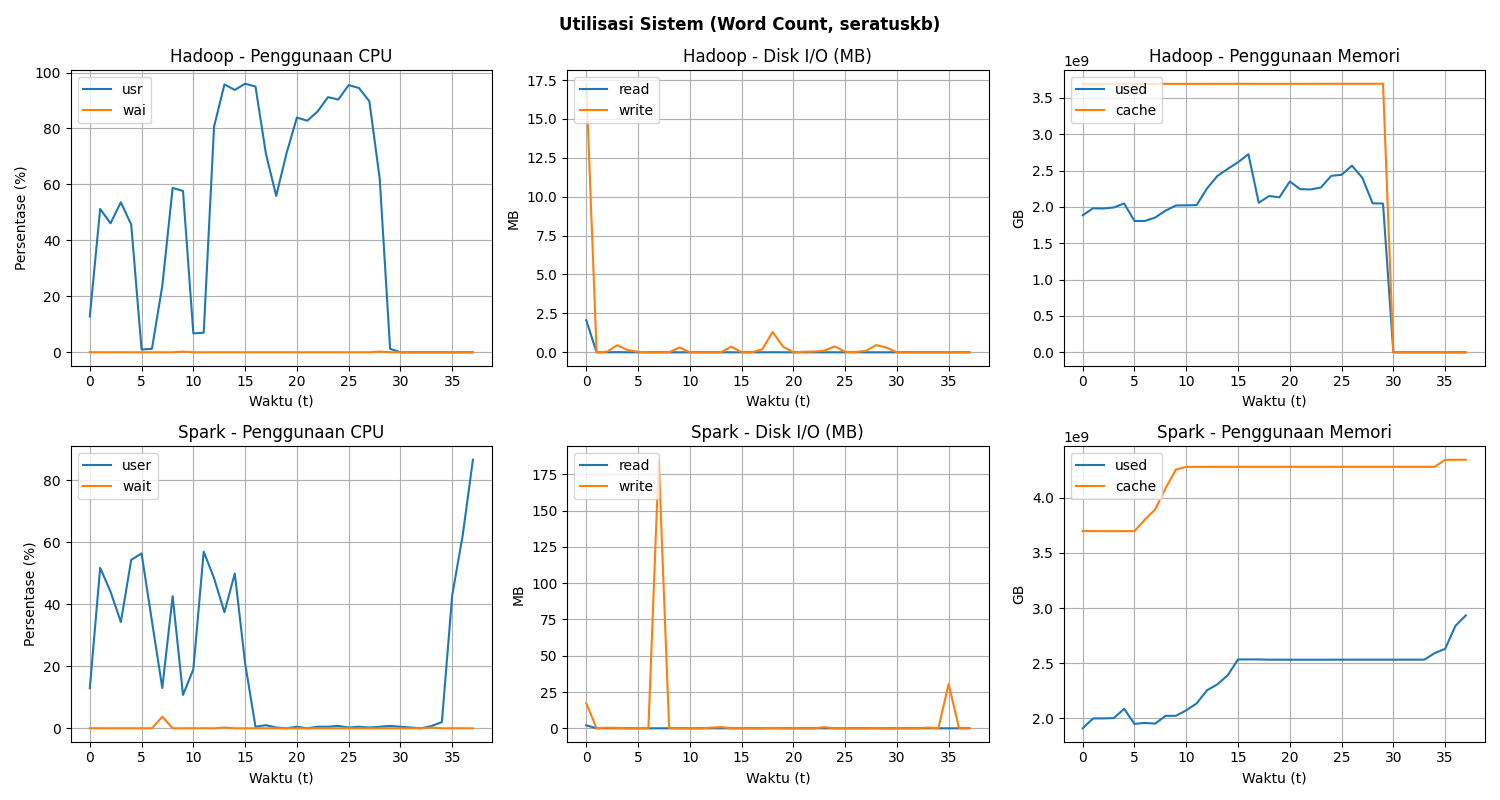
\includegraphics[width=1\textwidth]{figures/ch04/5-util-sistem-wordcount-seratuskb}
    \caption{Utilisasi Sistem (Word Count) pada Input Data 100 KB}
    \label{fig:5-util-sistem-wordcount-seratuskb}
\end{figure}

%\subsubsection{Input Data 500 KB}
%\blindtext
%\begin{figure}[h]
%    \centering
%    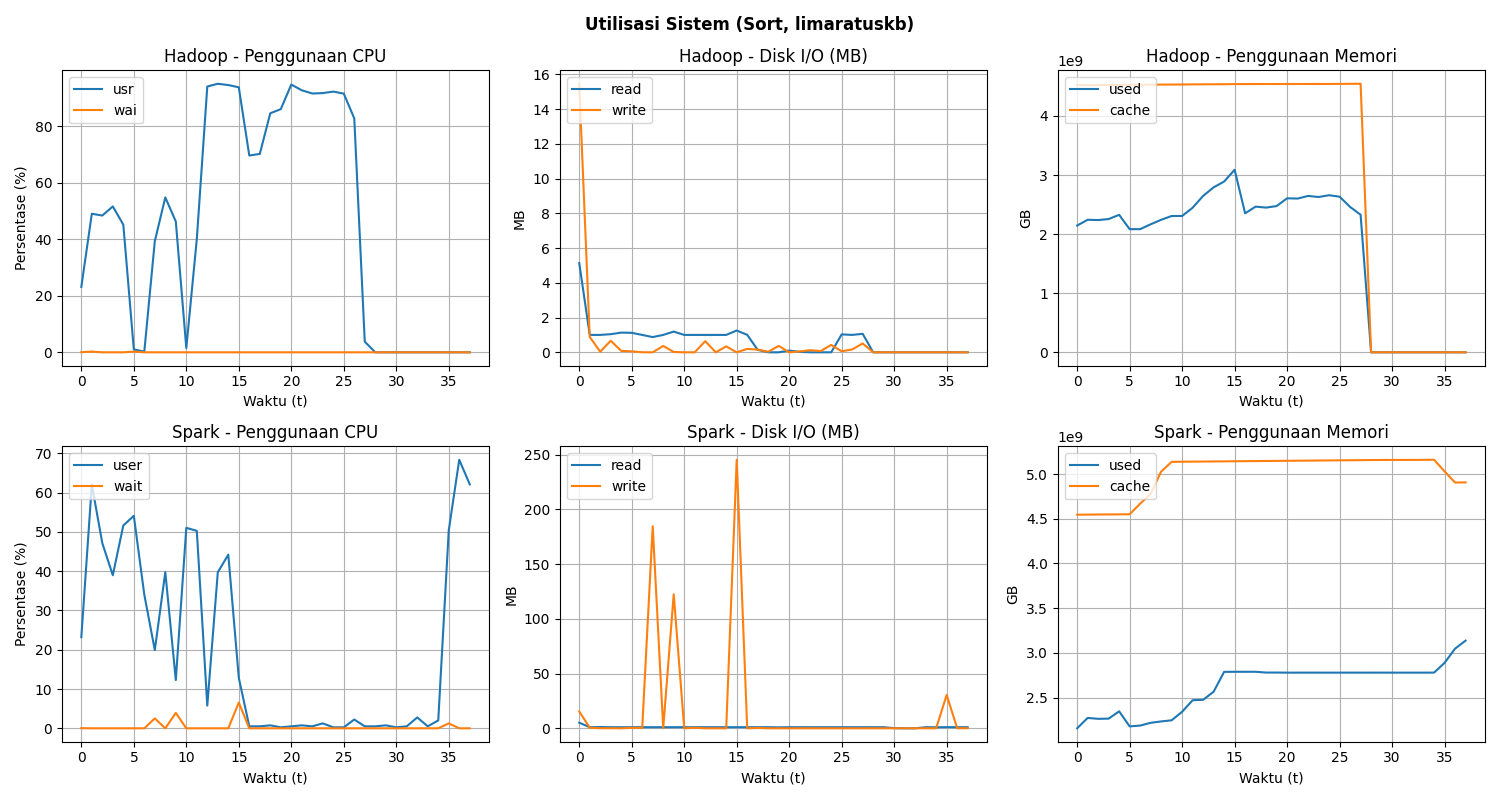
\includegraphics[width=1\textwidth]{figures/ch04/5-util-sistem-sort-limaratuskb}
%    \caption{Utilisasi Sistem (Sort) pada Input Data 500 KB}
%    \label{fig:5-util-sistem-sort-limaratuskb}
%\end{figure}
%
%\begin{figure}[h]
%    \centering
%    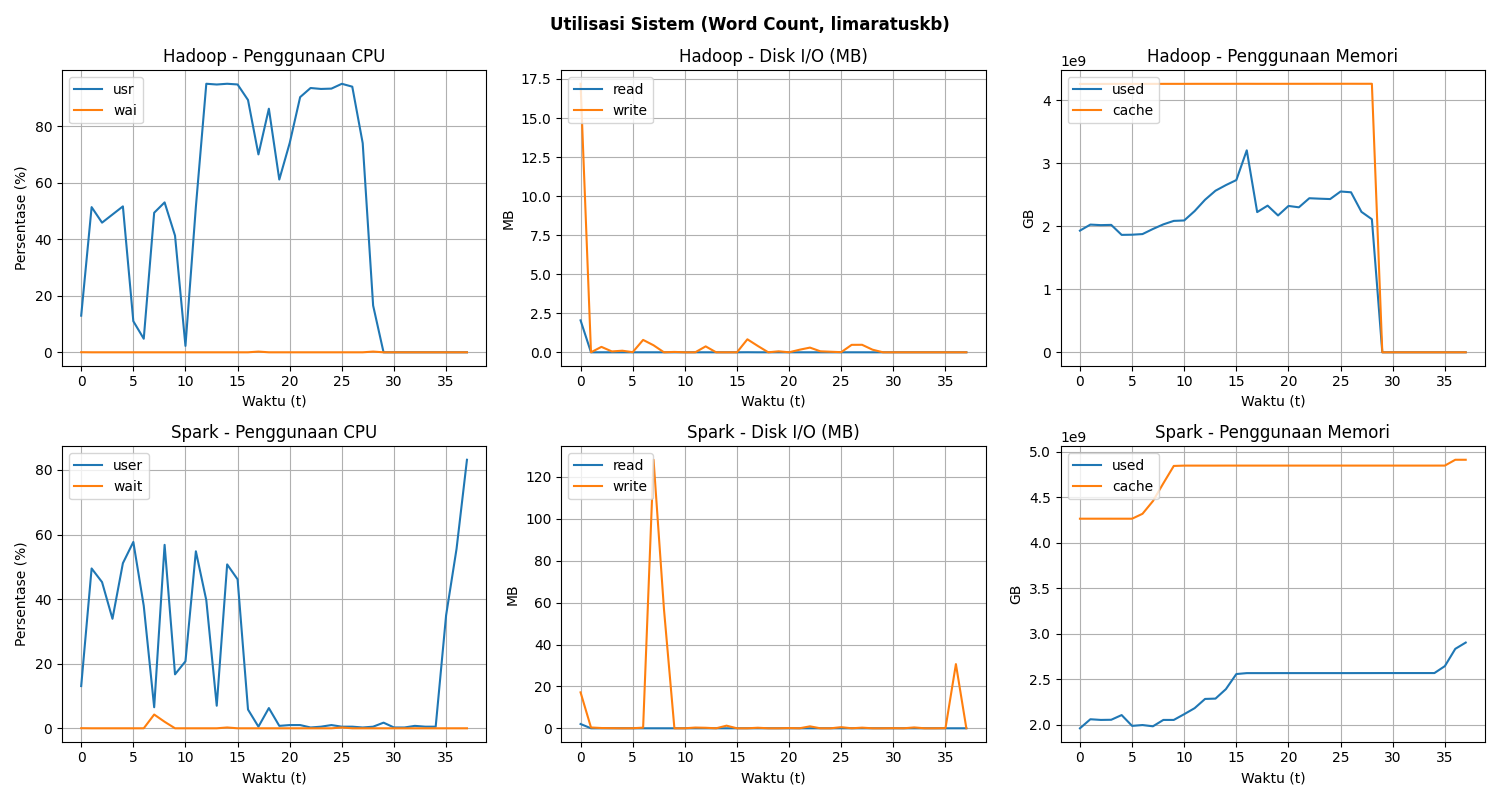
\includegraphics[width=1\textwidth]{figures/ch04/5-util-sistem-wordcount-limaratuskb}
%    \caption{Utilisasi Sistem (Word Count) pada Input Data 500 KB}
%    \label{fig:5-util-sistem-wordcount-limaratuskb}
%\end{figure}
%
%\subsubsection{Input Data 10 GB}
%\blindtext
%\begin{figure}[h]
%    \centering
%    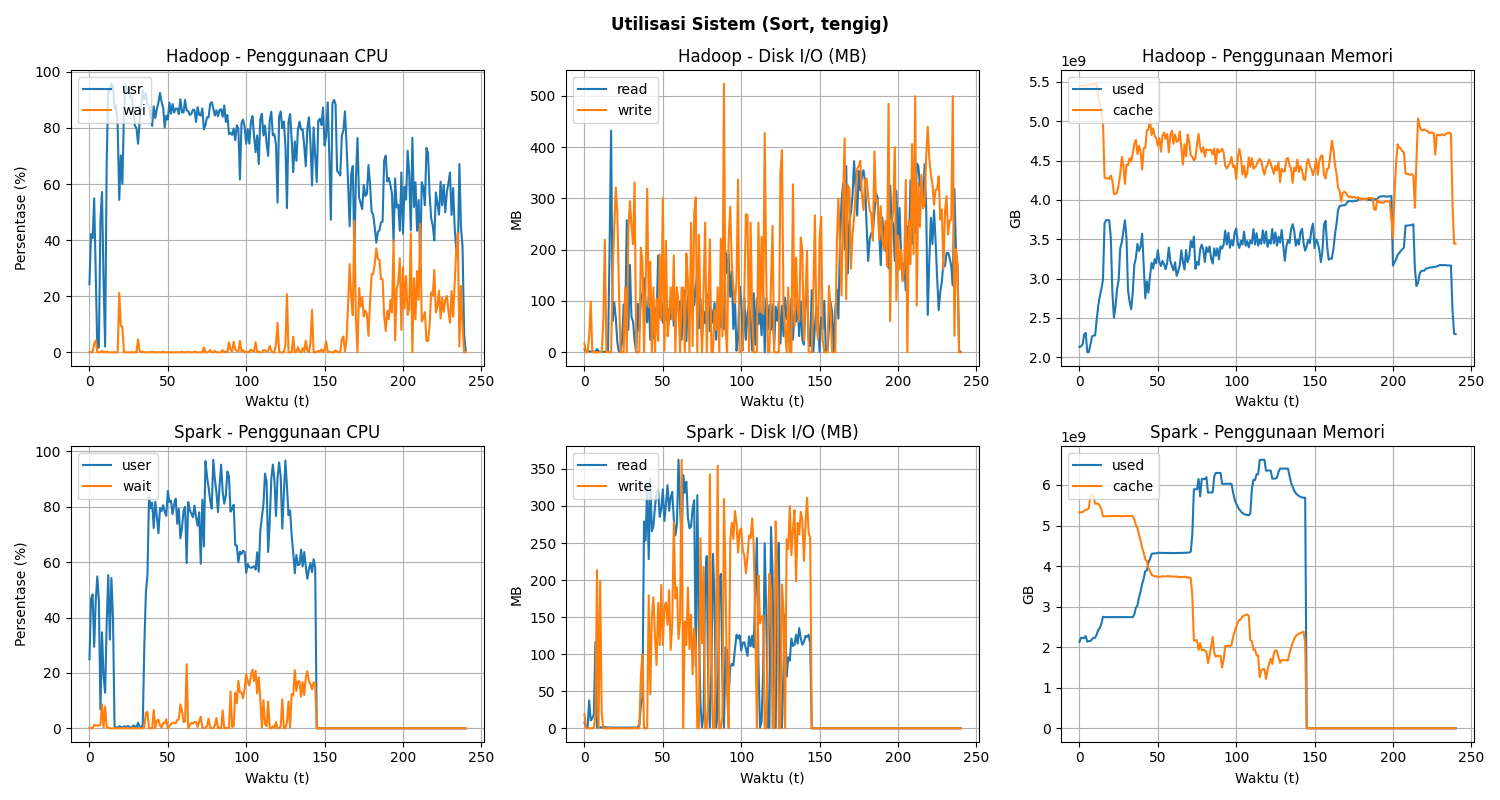
\includegraphics[width=1\textwidth]{figures/ch04/5-util-sistem-sort-tengig}
%    \caption{Utilisasi Sistem (Sort) pada Input Data 10 GB}
%    \label{fig:5-util-sistem-sort-tengig}
%\end{figure}
%
%\begin{figure}[h]
%    \centering
%    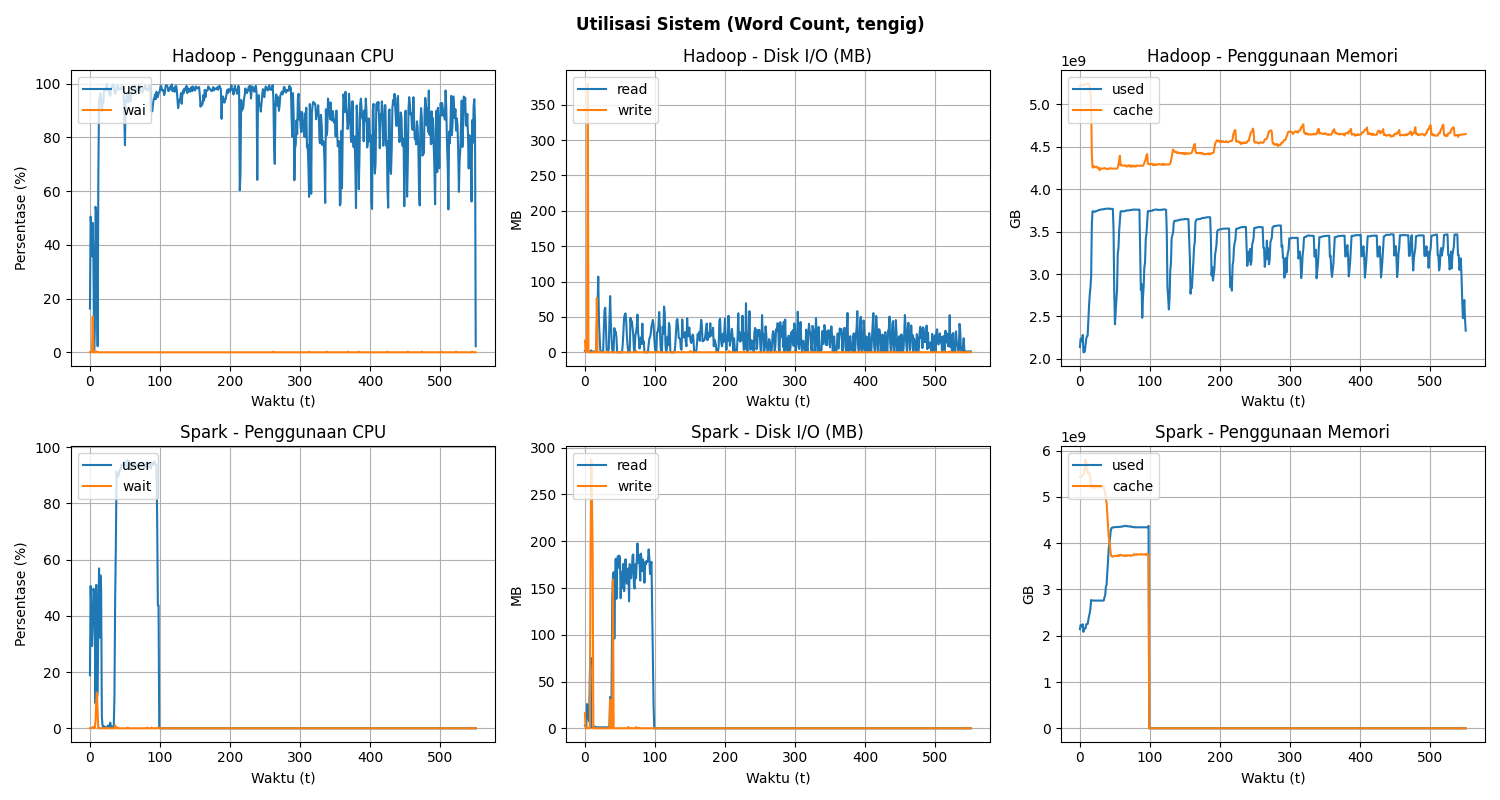
\includegraphics[width=1\textwidth]{figures/ch04/5-util-sistem-wordcount-tengig}
%    \caption{Utilisasi Sistem (Word Count) pada Input Data 10 GB}
%    \label{fig:5-util-sistem-wordcount-tengig}
%\end{figure}

\subsubsection{Input Data 15 GB}
\begin{figure}[h]
    \centering
    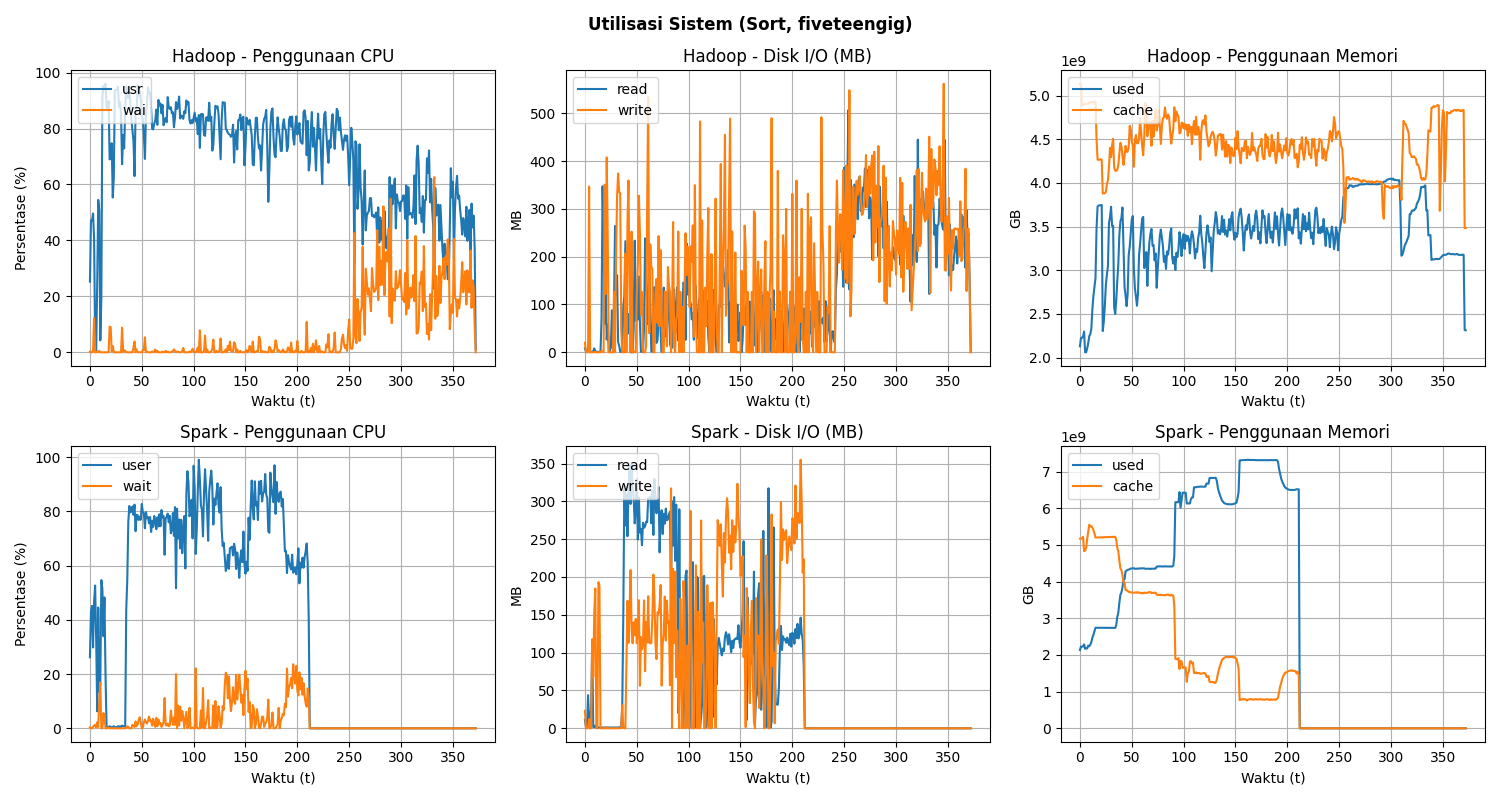
\includegraphics[width=1\textwidth]{figures/ch04/5-util-sistem-sort-fiveteengig}
    \caption{Utilisasi Sistem (Sort) pada Input Data 15 GB}
    \label{fig:5-util-sistem-sort-fiveteengig}
\end{figure}

\begin{figure}[h]
    \centering
    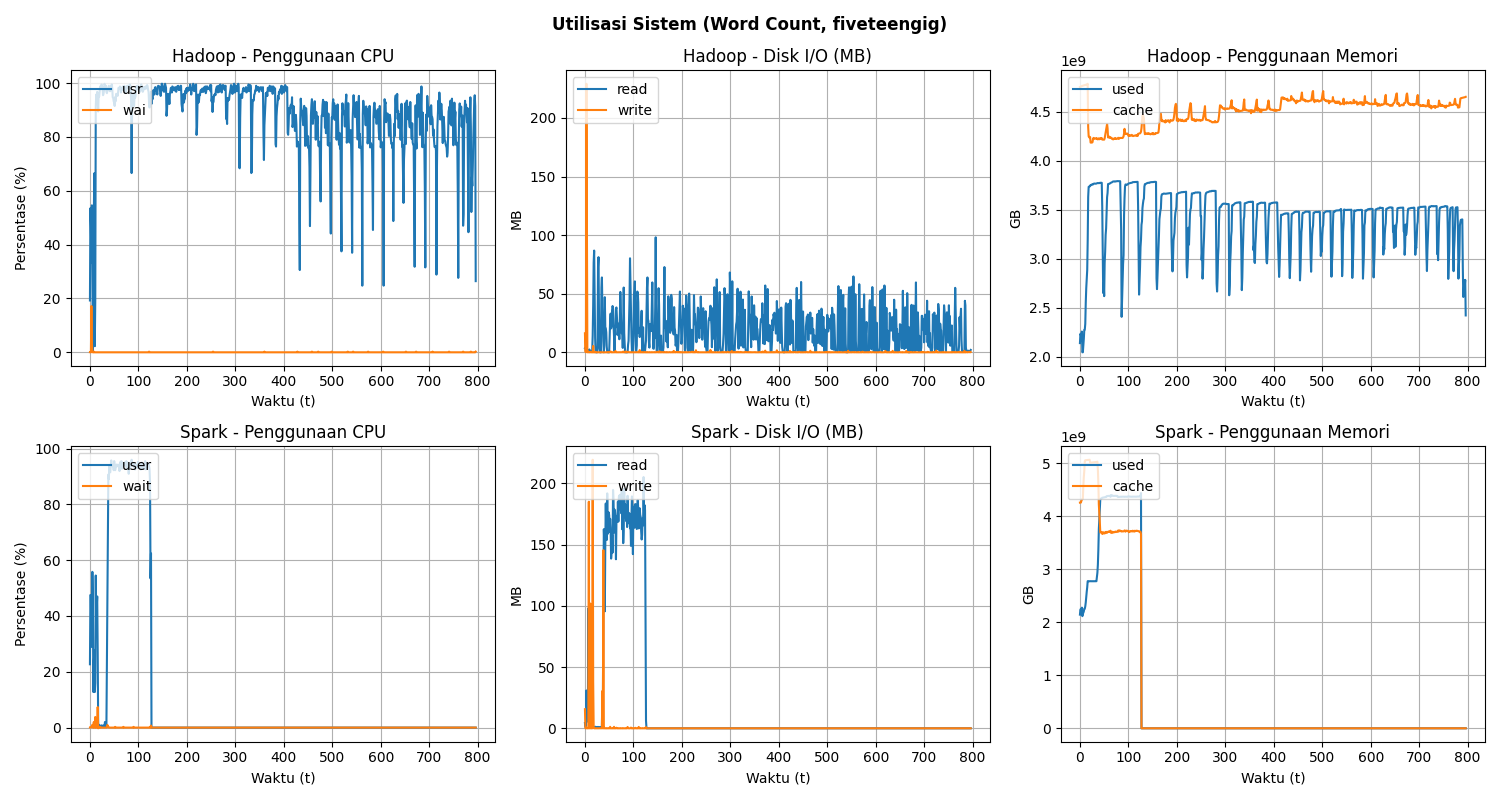
\includegraphics[width=1\textwidth]{figures/ch04/5-util-sistem-wordcount-fiveteengig}
    \caption{Utilisasi Sistem (Word Count) pada Input Data 15 GB}
    \label{fig:5-util-sistem-wordcount-fiveteengig}
\end{figure}


%\begin{landscape}
%\begin{longtable}{lllllrlrr}
%\toprule
% & Tanggal & Waktu & Jenis Beban Kerja & Aplikasi & Pengujian Ke- & Input Data & Waktu Eksekusi (detik) & Throughput (MB/s) \\
%\midrule
%1 & 17/04/24 & 10.07.03 & Wordcount & Hadoop & 1 & 100 KB & 27.192000 & 0.003731 \\
%2 & 17/04/24 & 10.07.33 & Wordcount & Hadoop & 2 & 100 KB & 27.308000 & 0.003715 \\
%3 & 17/04/24 & 10.08.02 & Wordcount & Hadoop & 3 & 100 KB & 26.364000 & 0.003848 \\
%4 & 17/04/24 & 10.08.32 & Wordcount & Hadoop & 4 & 100 KB & 27.184000 & 0.003732 \\
%5 & 17/04/24 & 10.09.02 & Wordcount & Hadoop & 5 & 100 KB & 28.186000 & 0.003599 \\
%... & ... & ... & ... & ... & ... & ... & ... & ... \\
%\bottomrule
%\end{tabular}
%\end{landscape}